% ============================================================
%  Network Security -- Module 4: Malicious Software
%  Lesson 6: Viruses, Worms and Trojan Horses
%  Beamer (Madrid theme). Compile with: pdflatex module4.tex (twice)
% ============================================================
\documentclass[aspectratio=169,11pt,xcolor={table}]{beamer}
\usetheme{Madrid}
\usefonttheme{professionalfonts}

\usepackage[T1]{fontenc}
\usepackage{lmodern}
\usepackage{booktabs}
\usepackage{array}
\usepackage{tikz}
\usetikzlibrary{arrows.meta,positioning,shapes.geometric,shapes.symbols,
  shapes.misc,shadows,calc,fit,backgrounds,mindmap,decorations.pathmorphing,decorations.pathreplacing}

% ------------------------------------------------------------
%  Colour palette
% ------------------------------------------------------------
\definecolor{navy}{RGB}{21,45,99}
\definecolor{ocean}{RGB}{28,97,158}
\definecolor{aqua}{RGB}{0,142,150}
\definecolor{brick}{RGB}{200,55,45}
\definecolor{amber}{RGB}{235,150,20}
\definecolor{leaf}{RGB}{40,160,90}
\definecolor{grape}{RGB}{125,70,165}
\definecolor{sky}{RGB}{235,243,252}
\definecolor{ink}{RGB}{40,40,50}

\setbeamercolor{palette primary}{bg=ocean,fg=white}
\setbeamercolor{palette secondary}{bg=navy!85,fg=white}
\setbeamercolor{palette tertiary}{bg=navy,fg=white}
\setbeamercolor{palette quaternary}{bg=navy,fg=white}
\setbeamercolor{structure}{fg=ocean}
\setbeamercolor{title}{bg=navy,fg=white}
\setbeamercolor{frametitle}{bg=navy,fg=white}
\setbeamercolor{block title}{bg=ocean,fg=white}
\setbeamercolor{block body}{bg=sky,fg=ink}
\setbeamercolor{block title alerted}{bg=brick,fg=white}
\setbeamercolor{block body alerted}{bg=brick!8,fg=ink}
\setbeamercolor{block title example}{bg=leaf,fg=white}
\setbeamercolor{block body example}{bg=leaf!8,fg=ink}
\setbeamercolor{normal text}{fg=ink}
\setbeamercolor{alerted text}{fg=brick}
\setbeamercolor{item projected}{bg=ocean,fg=white}
\setbeamertemplate{items}[circle]
\setbeamertemplate{blocks}[rounded][shadow=true]
\setbeamertemplate{navigation symbols}{}

% Section divider slide
\AtBeginSection[]{
  \begin{frame}[plain]
    \begin{tikzpicture}[remember picture,overlay]
      \fill[navy] (current page.south west) rectangle (current page.north east);
      \fill[ocean] (current page.south west) rectangle ([yshift=1.2cm]current page.south east);
      \fill[aqua] ([yshift=1.2cm]current page.south west) rectangle ([yshift=1.35cm]current page.south east);
      \foreach \i in {1,...,6}
        \draw[white,opacity=0.06,line width=14pt]
          ([xshift=\i*1.6cm]current page.north west) circle (\i*0.9cm);
      \node[white,font=\large,anchor=west] at ([xshift=1.2cm,yshift=0.9cm]current page.west)
        {Lesson \thesection};
      \node[white,font=\huge\bfseries,anchor=west,text width=12cm] at ([xshift=1.2cm,yshift=-0.1cm]current page.west)
        {\insertsectionhead};
      \node[white,opacity=0.8,anchor=east,font=\small] at ([xshift=-0.8cm,yshift=0.6cm]current page.south east)
        {Module 4 \,$\cdot$\, Malicious Software};
    \end{tikzpicture}
  \end{frame}
}

% ------------------------------------------------------------
%  TikZ styles and small pictograms
% ------------------------------------------------------------
\tikzset{
  >={Stealth[length=2.6mm]},
  box/.style={draw=#1!80!black,fill=#1!15,rounded corners=4pt,thick,
    minimum height=8mm,minimum width=22mm,align=center,font=\small,
    drop shadow={opacity=0.25}},
  box/.default=ocean,
  lay/.style={fill=#1,text=white,rounded corners=3pt,minimum width=38mm,minimum height=9mm,font=\scriptsize,align=center},
  solid box/.style={fill=#1,text=white,rounded corners=4pt,
    minimum height=8mm,minimum width=22mm,align=center,font=\small\bfseries,
    drop shadow={opacity=0.3}},
  solid box/.default=ocean,
  flow/.style={->,very thick,draw=#1},
  flow/.default=ink!70,
  station/.style={circle,draw=#1!80!black,fill=#1!20,very thick,minimum size=13mm,
    font=\small\bfseries,align=center},
  station/.default=ocean,
  tag/.style={font=\scriptsize,text=ink!80,align=center},
  layer/.style={draw=white,thick,fill=#1,text=white,minimum width=40mm,
    minimum height=6.5mm,font=\small\bfseries},
  % pictograms
  pics/pc/.style={code={
    \fill[#1!85!black,rounded corners=1.5pt] (-0.42,-0.05) rectangle (0.42,0.52);
    \fill[white!90!#1] (-0.36,0.01) rectangle (0.36,0.46);
    \fill[#1!85!black] (-0.06,-0.05) rectangle (0.06,-0.18);
    \fill[#1!85!black,rounded corners=1pt] (-0.24,-0.18) rectangle (0.24,-0.24);
  }},
  pics/pc/.default=ocean,
  pics/person/.style={code={
    \fill[#1] (0,0.46) circle (0.16);
    \fill[#1,rounded corners=5pt] (-0.27,-0.1) -- (-0.27,0.2) -- (0.27,0.2) -- (0.27,-0.1) -- cycle;
  }},
  pics/person/.default=ocean,
  pics/lock/.style={code={
    \draw[#1!80!black,line width=2.2pt] (-0.15,0.12) -- (-0.15,0.28) arc (180:0:0.15) -- (0.15,0.12);
    \fill[#1,rounded corners=2pt] (-0.26,-0.22) rectangle (0.26,0.14);
    \fill[white] (0,-0.02) circle (0.05);
    \fill[white] (-0.02,-0.02) rectangle (0.02,-0.13);
  }},
  pics/lock/.default=amber,
  pics/doc/.style={code={
    \fill[white,draw=#1,thick] (-0.25,-0.33) -- (-0.25,0.33) -- (0.12,0.33) -- (0.25,0.2) -- (0.25,-0.33) -- cycle;
    \draw[#1,thick] (0.12,0.33) -- (0.12,0.2) -- (0.25,0.2);
    \foreach \y in {0.12,0,-0.12,-0.24} \draw[#1!70,thick] (-0.16,\y) -- (0.16,\y);
  }},
  pics/doc/.default=ocean,
  pics/key/.style={code={
    \draw[#1,line width=2pt] (0,0) circle (0.12);
    \draw[#1,line width=2pt] (0.12,0) -- (0.5,0) (0.38,0) -- (0.38,-0.12) (0.47,0) -- (0.47,-0.1);
  }},
  pics/key/.default=amber,
}
\newcommand{\comma}{,}
\newcommand{\hl}[1]{\textcolor{ocean}{\textbf{#1}}}
\newcommand{\bad}[1]{\textcolor{brick}{\textbf{#1}}}
\newcommand{\good}[1]{\textcolor{leaf}{\textbf{#1}}}

\makeatletter
% University logo, small, top-right corner of every page
\AddToHook{shipout/foreground}{%
  \put(\strip@pt\paperwidth,0){%
    \makebox(0,0)[tr]{\raisebox{-0.8cm}{
\includegraphics[height=0.72cm]{au_logo.png}\hspace{0.15cm}}}}}
\makeatother

% ------------------------------------------------------------
\title[Module 4: Malicious Software]{Malicious Software}
\subtitle{Module 4 \,\textbar\, Lesson 6: Viruses, Worms and Trojan Horses}
\author[Network Security]{Network Security}
\institute[SLM]{Self-Learning Material \,--\, Lesson 6}
\date{}

% small bug pictogram
\tikzset{pics/bug/.style={code={
  \fill[#1] (0,0) ellipse (0.22 and 0.3);
  \fill[#1] (0,0.36) circle (0.13);
  \foreach \s in {-1,1}{
    \draw[#1,line width=1.2pt] (\s*0.18,0.12) -- (\s*0.42,0.24);
    \draw[#1,line width=1.2pt] (\s*0.2,-0.02) -- (\s*0.45,-0.02);
    \draw[#1,line width=1.2pt] (\s*0.18,-0.16) -- (\s*0.42,-0.3);
    \draw[#1,line width=1pt] (\s*0.06,0.46) -- (\s*0.16,0.62);
  }
  \draw[white,line width=0.8pt] (0,0.26) -- (0,-0.28);
}},pics/bug/.default=brick}

\begin{document}

% ============================================================
\begin{frame}[plain]
  
\begin{tikzpicture}[remember picture,overlay]
    \shade[top color=navy,bottom color=ocean] (current page.south west) rectangle (current page.north east);
    \foreach \i/\o in {1/0.10,2/0.08,3/0.06,4/0.05,5/0.04}
      \draw[white,opacity=\o,line width=1.2pt] ([xshift=-2.5cm,yshift=-0.5cm]current page.north east) circle (\i*1.1cm);
    \fill[aqua] ([yshift=2.35cm]current page.south west) rectangle ([yshift=2.45cm]current page.south east);
    \begin{scope}[shift={([xshift=-3.0cm,yshift=0.4cm]current page.east)}]
      \fill[white,opacity=0.9,rounded corners=4pt] (-1.3,-0.9) rectangle (1.3,1.0);
      \fill[ocean!70] (-1.15,-0.75) rectangle (1.15,0.85);
      \fill[white,opacity=0.9] (-0.15,-0.9) rectangle (0.15,-1.25);
      \fill[white,opacity=0.9,rounded corners=2pt] (-0.6,-1.25) rectangle (0.6,-1.38);
      \pic[scale=1.6] at (0,0.0) {bug=brick};
      \pic[scale=0.7] at (-1.75,1.0) {bug=white};
      \pic[scale=0.6] at (1.8,-0.6) {bug=white};
    \end{scope}
    \node[white,anchor=west,font=\normalsize] at ([xshift=1.1cm,yshift=2.4cm]current page.west)
      {NETWORK SECURITY \,\textbar\, MODULE 4};
    \node[white,anchor=west,font=\fontsize{30}{36}\selectfont\bfseries,text width=9.5cm] at ([xshift=1.1cm,yshift=1.1cm]current page.west)
      {Malicious Software};
    \node[white,opacity=0.9,anchor=west,text width=9cm,font=\small] at ([xshift=1.1cm,yshift=-0.4cm]current page.west)
      {Lesson 6 \,--\, Viruses, Worms and Trojan Horses};
    \node[white,opacity=0.85,anchor=west,font=\footnotesize] at ([xshift=1.1cm,yshift=1.2cm]current page.south west)
      {Bombs \,$\cdot$\, Trojans \,$\cdot$\, Worms \,$\cdot$\, Viruses \,$\cdot$\, Infection \,$\cdot$\, Prevention \,$\cdot$\, Cure \,$\cdot$\, Hardening};
  \end{tikzpicture}
\end{frame}

% ============================================================
\begin{frame}{Roadmap of This Module}
  \centering
  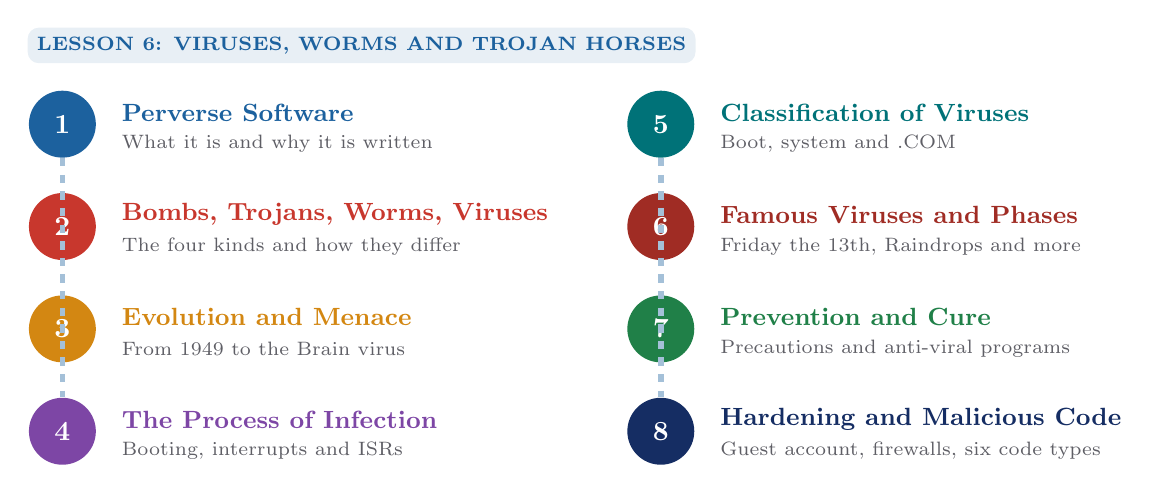
\begin{tikzpicture}
    \foreach \t/\c/\n [count=\i] in {
      Perverse Software/ocean/What it is and why it is written,
      Bombs\comma{} Trojans\comma{} Worms\comma{} Viruses/brick/The four kinds and how they differ,
      Evolution and Menace/amber!90!black/From 1949 to the Brain virus,
      The Process of Infection/grape/Booting\comma{} interrupts and ISRs,
      Classification of Viruses/aqua!80!black/Boot\comma{} system and .COM/.EXE infectors,
      Famous Viruses and Phases/brick!80!black/Friday the 13th\comma{} Raindrops and more,
      Prevention and Cure/leaf!80!black/Precautions and anti-viral programs,
      Hardening and Malicious Code/navy/Guest account\comma{} firewalls\comma{} six code types}
    {
      \pgfmathsetmacro{\x}{ifthenelse(\i<5,0,7.6)}
      \pgfmathsetmacro{\y}{-mod(\i-1,4)*1.3}
      \node[circle,fill=\c,text=white,font=\bfseries,minimum size=8.5mm] (n\i) at (\x,\y) {\i};
      \node[anchor=west,font=\small\bfseries,text=\c] at ([xshift=2mm,yshift=1.5mm]n\i.east) {\t};
      \node[anchor=west,font=\scriptsize,text=ink!75] at ([xshift=2mm,yshift=-2.5mm]n\i.east) {\n};
    }
    \draw[ocean!40,line width=2pt,dashed] (n1) -- (n4);
    \draw[ocean!40,line width=2pt,dashed] (n5) -- (n8);
    \node[fill=ocean!10,rounded corners,font=\scriptsize\bfseries,text=ocean] at (3.8,1.0) {LESSON 6: VIRUSES, WORMS AND TROJAN HORSES};
  \end{tikzpicture}
\end{frame}

% ============================================================
\setcounter{section}{5}
\section{Viruses, Worms and Trojan Horses}
% ============================================================

\begin{frame}{What You Will Learn}
  \begin{columns}[c]
    \begin{column}{0.52\textwidth}
      \centering
      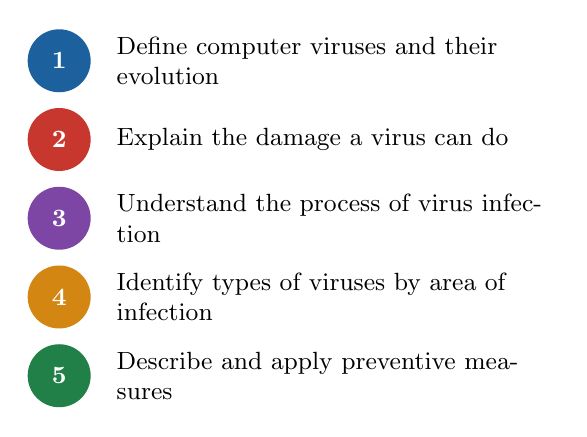
\begin{tikzpicture}
        \foreach \t/\c [count=\i from 0] in {Define computer viruses and their evolution/ocean,Explain the damage a virus can do/brick,Understand the process of virus infection/grape,Identify types of viruses by area of infection/amber!90!black,Describe and apply preventive measures/leaf!80!black}{
          \node[circle,fill=\c,text=white,font=\small\bfseries,minimum size=8mm] (c\i) at (0,-\i*1.0) {\the\numexpr\i+1\relax};
          \node[anchor=west,font=\small,text width=55mm] at ([xshift=2mm]c\i.east) {\t};
        }
      \end{tikzpicture}
    \end{column}
    \begin{column}{0.46\textwidth}
      \begin{alertblock}{An era of electronic terrorism}
        \small The world of IT is going through an era of electronic terrorism in the form of viruses, a problem dangerous enough to \textbf{threaten the proper functioning} of computer systems.
      \end{alertblock}
      \vspace{2mm}
      \begin{block}{Our plan}
        \small Evolution \,$\rightarrow$\, menace \,$\rightarrow$\, infection \,$\rightarrow$\, classification \,$\rightarrow$\, types \,$\rightarrow$\, prevention \,$\rightarrow$\, cure
      \end{block}
    \end{column}
  \end{columns}
\end{frame}

% ------------------------------------------------------------
\begin{frame}{What Is Perverse Software?}
  \begin{columns}[c]
    \begin{column}{0.5\textwidth}
      \centering
      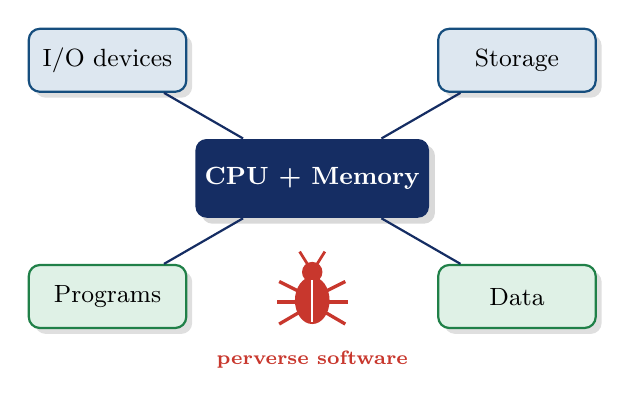
\begin{tikzpicture}
        \node[solid box=navy,minimum width=26mm,minimum height=10mm] (cpu) at (0,0) {CPU + Memory};
        \node[box=ocean,minimum width=20mm] (io) at (-2.6,1.5) {I/O devices};
        \node[box=ocean,minimum width=20mm] (st) at (2.6,1.5) {Storage};
        \node[box=leaf,minimum width=20mm] (pr) at (-2.6,-1.5) {Programs};
        \node[box=leaf,minimum width=20mm] (dt) at (2.6,-1.5) {Data};
        \foreach \n in {io,st,pr,dt} \draw[navy,thick] (cpu) -- (\n);
        \pic[scale=1.0] at (0,-1.55) {bug=brick};
        \node[font=\scriptsize\bfseries,text=brick] at (0,-2.3) {perverse software};
      \end{tikzpicture}
    \end{column}
    \begin{column}{0.48\textwidth}
      \begin{block}{Definition}
        \small ``Software which causes a \textbf{perverse activity}.''
      \end{block}
      \textbf{Perverse activities include:}
      \begin{itemize}\small\setlength{\itemsep}{2pt}
        \item Modifying or completely \textbf{destroying data} without the user's intention
        \item \textbf{Unpredictable behaviour} in display, print, etc.
        \item \textbf{Sabotaging} the operating system
      \end{itemize}
      \vspace{1mm}
      {\small A system running perverse software is called an \textbf{infected system}.}
    \end{column}
  \end{columns}
\end{frame}

% ------------------------------------------------------------
\begin{frame}{Why Is Perverse Software Written?}
  \centering
  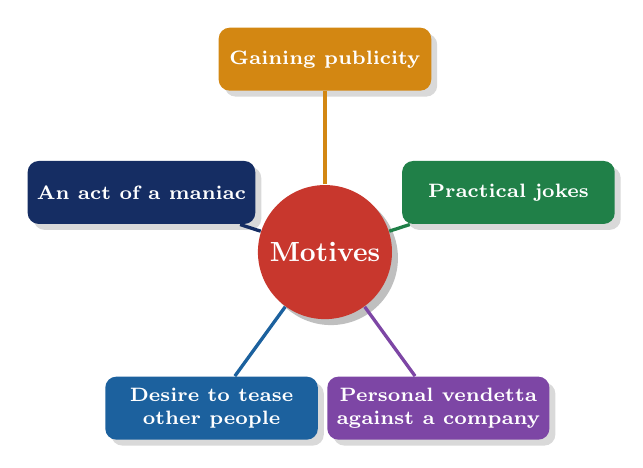
\begin{tikzpicture}
    \node[circle,fill=brick,text=white,font=\bfseries,minimum size=16mm,align=center,drop shadow] (c) at (0,0) {Motives};
    \foreach \a/\t/\c in {90/Gaining publicity/amber!90!black,18/Practical jokes/leaf!80!black,-54/Personal vendetta\\against a company/grape,-126/Desire to tease\\other people/ocean,162/An act of a maniac/navy}{
      \node[solid box=\c,minimum width=27mm,minimum height=8mm,font=\scriptsize\bfseries] (s\a) at (\a:2.45) {\t};
      \draw[\c,very thick] (c) -- (s\a);
    }
  \end{tikzpicture}
  \vspace{0mm}
  \begin{alertblock}{The result}
    \small All of them aim at producing \textbf{disastrous effects}, while the normal user only wants to do something \textbf{constructive} and increase productivity.
  \end{alertblock}
\end{frame}

% ------------------------------------------------------------
\begin{frame}{Why Is It So Hard to Notice?}
  \begin{columns}[c]
    \begin{column}{0.5\textwidth}
      \centering
      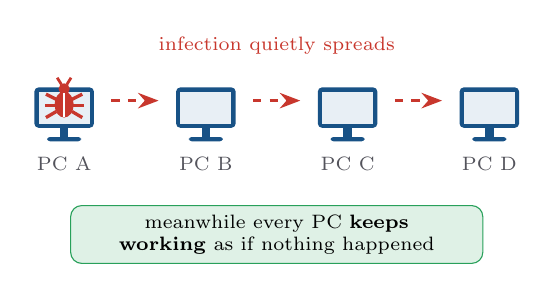
\begin{tikzpicture}
        \foreach \x/\l in {0/A,1.8/B,3.6/C,5.4/D}{
          \pic[scale=0.9] at (\x,0) {pc=ocean};
          \node[tag] at (\x,-0.5) {PC \l};
        }
        \pic[scale=0.55] at (0,0.25) {bug=brick};
        \foreach \x in {0.6,2.4,4.2} \draw[->,brick,very thick,dashed] (\x,0.3) -- (\x+0.6,0.3);
        \node[font=\scriptsize,text=brick] at (2.7,1.0) {infection quietly spreads};
        \node[fill=leaf!15,draw=leaf,rounded corners,font=\scriptsize,text width=50mm,align=center] at (2.7,-1.4) {meanwhile every PC \textbf{keeps working} as if nothing happened};
      \end{tikzpicture}
    \end{column}
    \begin{column}{0.48\textwidth}
      \begin{itemize}\small\setlength{\itemsep}{5pt}
        \item Different perverse software causes different activities, but all generate \textbf{uncertainty} for users
        \item Normal MS-DOS operations were designed for \textbf{bona fide users}, not to detect such software
        \item Standard security checks \textbf{do not detect} the anomaly
        \item So an infected system \textbf{continues to work}, spreading the infection
      \end{itemize}
    \end{column}
  \end{columns}
\end{frame}

% ------------------------------------------------------------
\begin{frame}{Four Kinds of Perverse Software}
  \centering
  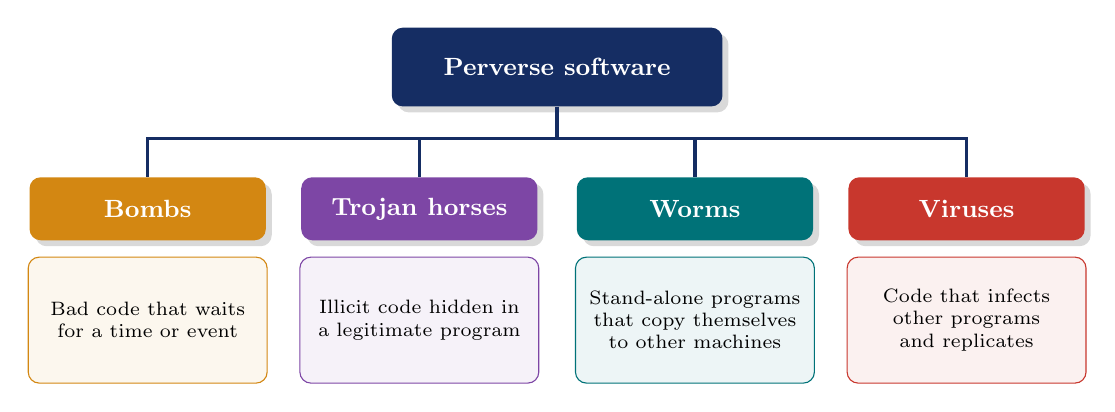
\begin{tikzpicture}
    \node[solid box=navy,minimum width=42mm,minimum height=10mm] (t) at (0,0) {Perverse software};
    \foreach \t/\c/\x/\d [count=\i] in {
      Bombs/amber!90!black/-5.2/Bad code that waits for a time or event,
      Trojan horses/grape/-1.75/Illicit code hidden in a legitimate program,
      Worms/aqua!80!black/1.75/Stand-alone programs that copy themselves to other machines,
      Viruses/brick/5.2/Code that infects other programs and replicates}
    {
      \node[solid box=\c,minimum width=30mm] (n\i) at (\x,-1.8) {\t};
      \draw[navy,very thick] (t.south) -- ++(0,-0.4) -| (n\i.north);
      \node[draw=\c,fill=\c!7,rounded corners,text width=28mm,minimum height=16mm,align=center,font=\scriptsize,anchor=north] at ([yshift=-2mm]n\i.south) {\d};
    }
  \end{tikzpicture}
  \vspace{3mm}
  \begin{block}{Note}
    \small In everyday speech ``virus'' is a very broad term that also includes worms and Trojans. In this lesson we keep them separate.
  \end{block}
\end{frame}

% ------------------------------------------------------------
\begin{frame}{(a) Bombs}
  \begin{columns}[c]
    \begin{column}{0.45\textwidth}
      \centering
      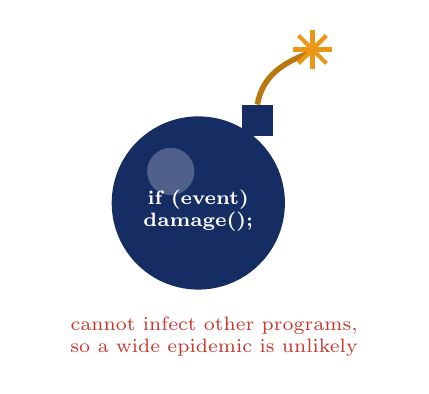
\begin{tikzpicture}
        \fill[navy] (0,0) circle (1.1);
        \fill[white,opacity=0.25] (-0.35,0.4) circle (0.3);
        \fill[navy] (0.55,0.85) rectangle (0.95,1.25);
        \draw[amber!80!black,line width=2pt] (0.75,1.25) to[out=80,in=200] (1.4,1.9);
        \foreach \a in {0,45,...,315} \draw[amber,line width=1.5pt] (1.45,1.95) -- ++(\a:0.25);
        \node[white,font=\scriptsize\bfseries,align=center] at (0,-0.1) {if (event)\\ damage();};
        \node[font=\scriptsize,text=brick,text width=45mm,align=center] at (0.2,-1.7) {cannot infect other programs, so a wide epidemic is unlikely};
      \end{tikzpicture}
    \end{column}
    \begin{column}{0.52\textwidth}
      \begin{block}{Definition}
        \small A piece of \textbf{bad code deliberately planted} by an insider or supplier of a program.
      \end{block}
      \begin{itemize}\small\setlength{\itemsep}{3pt}
        \item \textbf{Triggered} by an event that is logical or time based
        \item ``Explodes'' when the conditions are met, causing damage \textbf{immediately}
        \item \textbf{Cannot infect other programs}, so it does not propagate
        \item Two types: \textbf{time bombs} and \textbf{logic bombs}
      \end{itemize}
    \end{column}
  \end{columns}
\end{frame}

% ------------------------------------------------------------
\begin{frame}{Time Bomb vs.\ Logic Bomb}
  \begin{columns}[T]
    \begin{column}{0.49\textwidth}
      \centering\textbf{\textcolor{amber!80!black}{Time bomb}}\\[2mm]
      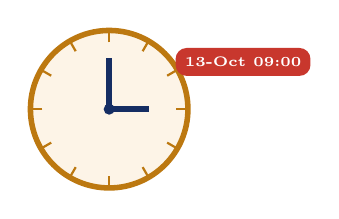
\begin{tikzpicture}
        \draw[amber!80!black,line width=2pt,fill=amber!10] (0,0) circle (1.0);
        \foreach \a in {0,30,...,330} \draw[amber!80!black,thick] (\a:0.85) -- (\a:1.0);
        \draw[navy,line width=2pt] (0,0) -- (90:0.65);
        \draw[navy,line width=2pt] (0,0) -- (0:0.5);
        \fill[navy] (0,0) circle (0.07);
        \node[fill=brick,text=white,font=\tiny\bfseries,rounded corners] at (1.7,0.6) {13-Oct 09:00};
      \end{tikzpicture}\\[2mm]
      {\small Named after its physical counterpart: it goes off at a \textbf{set date and time}, started by the \textbf{computer clock}. It may disrupt the system, modify or destroy stored data.}
    \end{column}
    \begin{column}{0.49\textwidth}
      \centering\textbf{\textcolor{grape}{Logic bomb}}\\[2mm]
      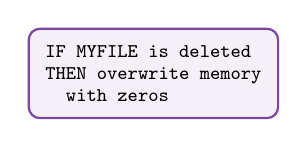
\begin{tikzpicture}
        \node[draw=grape,fill=grape!8,thick,rounded corners,font=\scriptsize\ttfamily,align=left,inner sep=6pt] {IF MYFILE is deleted\\THEN overwrite memory\\\quad with zeros};
      \end{tikzpicture}\\[4mm]
      {\small Activated by a \textbf{certain combination of events}. In the example, deleting a file called MYFILE destroys the contents of memory.}
    \end{column}
  \end{columns}
  \vspace{3mm}
  \begin{block}{Both types}
    \small Can be set to go off at a \textbf{future time or event}, and can be planted by someone with inside access.
  \end{block}
\end{frame}

% ------------------------------------------------------------
\begin{frame}{(b) Trojan Horse}
  \begin{columns}[c]
    \begin{column}{0.45\textwidth}
      \centering
      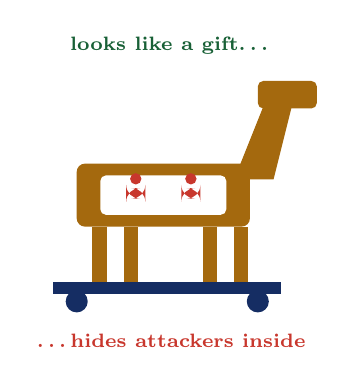
\begin{tikzpicture}
        % simple wooden horse
        \fill[amber!70!black,rounded corners=3pt] (-1.2,0) rectangle (1.0,0.8);
        \fill[amber!70!black] (0.8,0.6) -- (1.2,1.6) -- (1.55,1.6) -- (1.3,0.6) -- cycle;
        \fill[amber!70!black,rounded corners=2pt] (1.1,1.5) rectangle (1.85,1.85);
        \foreach \x in {-1.0,-0.6,0.4,0.8} \fill[amber!70!black] (\x,0) rectangle (\x+0.18,-0.7);
        \fill[navy] (-1.5,-0.85) rectangle (1.4,-0.7);
        \foreach \x in {-1.2,1.1} \fill[navy] (\x,-0.95) circle (0.14);
        \fill[white,rounded corners=2pt] (-0.9,0.15) rectangle (0.7,0.65);
        \pic[scale=0.45] at (-0.45,0.4) {person=brick};
        \pic[scale=0.45] at (0.25,0.4) {person=brick};
        \node[font=\scriptsize\bfseries,text=leaf!60!black] at (0,2.3) {looks like a gift\dots};
        \node[font=\scriptsize\bfseries,text=brick] at (0,-1.45) {\dots hides attackers inside};
      \end{tikzpicture}
    \end{column}
    \begin{column}{0.52\textwidth}
      \begin{block}{Definition}
        \small An \textbf{illicit coding} contained in a legitimate program, which causes an illegitimate action. Named after the wooden horse of Troy.
      \end{block}
      \begin{itemize}\small\setlength{\itemsep}{2pt}
        \item May change or steal \textbf{passwords}, or modify protected records
        \item Hides in a host and generally does \textbf{not damage the host}
        \item \textbf{Cannot copy itself} to other software
        \item Activated only when the illicit program is \textbf{called explicitly}
        \item Spreads only when an unsuspecting user \textbf{copies} the program
      \end{itemize}
    \end{column}
  \end{columns}
\end{frame}

% ------------------------------------------------------------
\begin{frame}{Example: The Christmas Card Trojan}
  \centering
  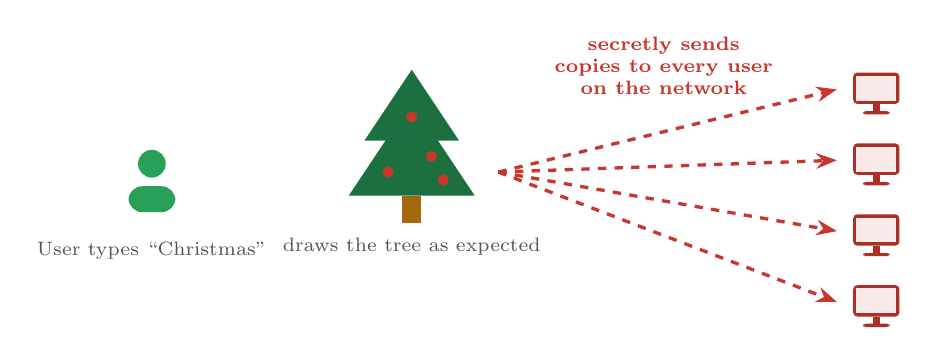
\begin{tikzpicture}
    \pic[scale=1.1] at (0,0) {person=leaf}; \node[tag] at (0,-0.6) {User types ``Christmas''};
    % tree
    \begin{scope}[shift={(3.3,0)}]
      \fill[leaf!70!black] (0,1.3) -- (-0.8,0.1) -- (0.8,0.1) -- cycle;
      \fill[leaf!70!black] (0,1.7) -- (-0.6,0.8) -- (0.6,0.8) -- cycle;
      \fill[amber!70!black] (-0.12,0.1) rectangle (0.12,-0.25);
      \foreach \p in {(-0.3,0.4),(0.25,0.6),(0,1.1),(0.4,0.3)} \fill[brick] \p circle (0.07);
      \node[tag] at (0,-0.55) {draws the tree as expected};
    \end{scope}
    \foreach \y [count=\i] in {1.3,0.4,-0.5,-1.4}{
      \pic[scale=0.7] at (9.2,\y) {pc=brick};
      \draw[->,brick,very thick,dashed] (4.4,0.4) -- (8.7,\y+0.15);
    }
    \node[font=\scriptsize\bfseries,text=brick,text width=30mm,align=center] at (6.5,1.75) {secretly sends copies to \textbf{every user} on the network};
  \end{tikzpicture}
  \vspace{3mm}
  \begin{alertblock}{What happened}
    \small Detected on IBM's internal e-mail. The program did what it promised, drawing a Christmas tree, but also flooded the network with copies. Other users could not even \textbf{save their half-finished work}.
  \end{alertblock}
\end{frame}

% ------------------------------------------------------------
\begin{frame}{(c) Worms}
  \begin{columns}[c]
    \begin{column}{0.5\textwidth}
      \centering
      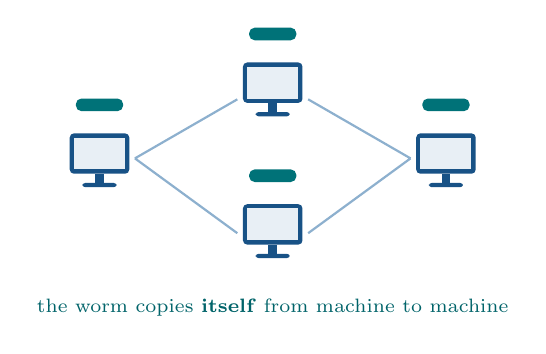
\begin{tikzpicture}
        \foreach \x/\y [count=\i] in {0/0,2.2/0.9,2.2/-0.9,4.4/0}{
          \pic[scale=0.9] at (\x,\y) {pc=ocean};
        }
        \draw[ocean!50,thick] (0.45,0.15) -- (1.75,0.9) (0.45,0.15) -- (1.75,-0.8) (2.65,0.9) -- (3.95,0.15) (2.65,-0.8) -- (3.95,0.15);
        \foreach \x/\y in {0/0.75,2.2/1.65,2.2/-0.15,4.4/0.75}
          \fill[aqua!80!black,rounded corners=2pt] (\x-0.3,\y) rectangle (\x+0.3,\y+0.16);
        \node[font=\scriptsize,text=aqua!70!black] at (2.2,-1.75) {the worm copies \textbf{itself} from machine to machine};
      \end{tikzpicture}
    \end{column}
    \begin{column}{0.48\textwidth}
      \begin{itemize}\small\setlength{\itemsep}{4pt}
        \item A worm can \textbf{relocate itself} and does \textbf{not need a host program}
        \item It copies itself to \textbf{another machine} on the network
        \item Worms are \textbf{stand-alone} programs, so they are easier to detect than Trojans and viruses
        \item Worms store themselves in critical disk areas and have been known to \textbf{damage entire LANs}
      \end{itemize}
      \vspace{1mm}
      \begin{block}{Worm vs.\ Trojan}
        \small A Trojan needs a host and cannot replicate; a worm needs no host and replicates.
      \end{block}
    \end{column}
  \end{columns}
\end{frame}

% ------------------------------------------------------------
\begin{frame}{Worms Can Also Be Useful}
  \begin{columns}[c]
    \begin{column}{0.5\textwidth}
      \begin{block}{Useful work}
        \small Worms can sabotage systems, but can also do \textbf{useful tasks}, for example installing a network. Insert a worm and check for it at each node: a node where it never appears can be assumed \textbf{not connected}.
      \end{block}
      \centering
      
\begin{tikzpicture}
        \foreach \x/\ok in {0/1,1.4/1,2.8/0,4.2/1}{
          \ifnum\ok=1
            \node[circle,fill=leaf,text=white,font=\scriptsize\bfseries,minimum size=8mm] at (\x,0) {\checkmark};
          \else
            \node[circle,fill=brick,text=white,font=\scriptsize\bfseries,minimum size=8mm] at (\x,0) {$\times$};
          \fi
        }
        \node[font=\tiny,text=brick] at (2.8,-0.65) {not connected};
      \end{tikzpicture}
    \end{column}
    \begin{column}{0.48\textwidth}
      \centering\textbf{\textcolor{aqua!70!black}{Two named examples}}\\[3mm]
      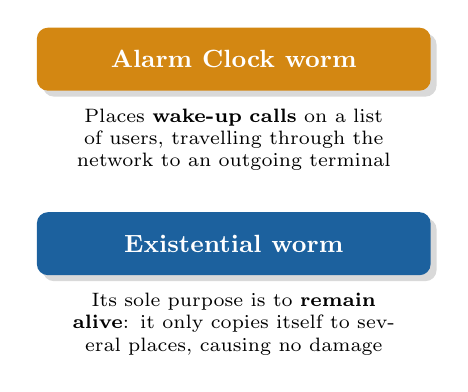
\begin{tikzpicture}
        \node[solid box=amber!90!black,minimum width=50mm] (a) at (0,0) {Alarm Clock worm};
        \node[font=\scriptsize,text width=50mm,align=center,below=1mm of a] (ad) {Places \textbf{wake-up calls} on a list of users, travelling through the network to an outgoing terminal};
        \node[solid box=ocean,minimum width=50mm,below=4mm of ad] (e) {Existential worm};
        \node[font=\scriptsize,text width=50mm,align=center,below=1mm of e] {Its sole purpose is to \textbf{remain alive}: it only copies itself to several places, causing no damage};
      \end{tikzpicture}
    \end{column}
  \end{columns}
\end{frame}

% ------------------------------------------------------------
\begin{frame}{(d) Viruses}
  \begin{columns}[c]
    \begin{column}{0.46\textwidth}
      \centering
      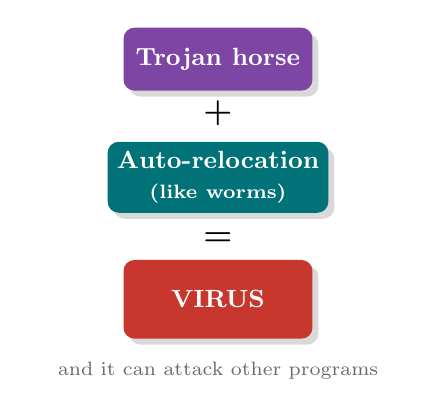
\begin{tikzpicture}
        \node[solid box=grape,minimum width=24mm] (t) at (0,1.5) {Trojan horse};
        \node[font=\large\bfseries] at (0,0.82) {+};
        \node[solid box=aqua!80!black,minimum width=24mm] (w) at (0,0) {Auto-relocation\\\scriptsize(like worms)};
        \node[font=\large\bfseries] at (0,-0.78) {=};
        \node[solid box=brick,minimum width=24mm,minimum height=10mm] (v) at (0,-1.55) {VIRUS};
        \node[font=\scriptsize,text=ink!70,text width=46mm,align=center] at (0,-2.45) {and it can attack other programs};
      \end{tikzpicture}
    \end{column}
    \begin{column}{0.52\textwidth}
      \begin{block}{Davis and Gantenbein (1987)}
        \small ``A Trojan horse program with the capability of \textbf{auto-relocation} (same as in worms) and it can \textbf{attack other programs}.''
      \end{block}
      \begin{itemize}\small\setlength{\itemsep}{2pt}
        \item The chronological \textbf{successor} of worm programs
        \item The \textbf{most dangerous} perverse software: it reproduces itself
        \item Attaches to a regularly used program so the host \textbf{looks benign}
        \item Highly \textbf{contagious}; can take control of the OS and destroy all data on the disk
      \end{itemize}
    \end{column}
  \end{columns}
\end{frame}

% ------------------------------------------------------------
\begin{frame}{A Virus Behaves Like a Parasite}
  \centering
  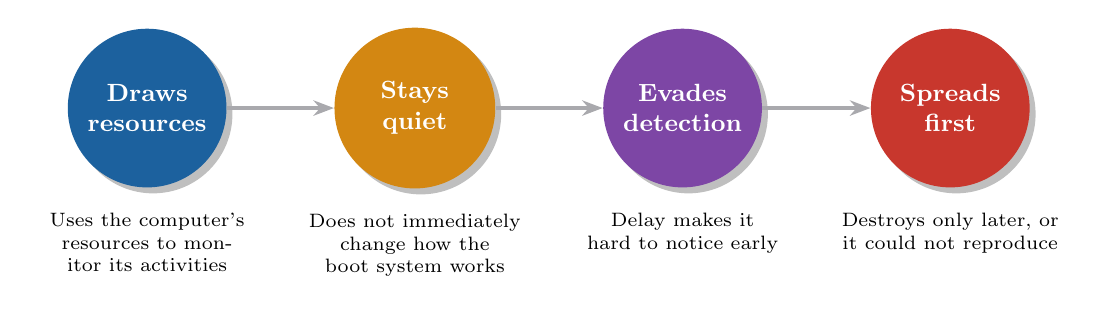
\begin{tikzpicture}
    \foreach \t/\d/\c [count=\i from 0] in {
      Draws resources/Uses the computer's resources to monitor its activities/ocean,
      Stays quiet/Does not immediately change how the boot system works/amber!90!black,
      Evades detection/Delay makes it hard to notice early/grape,
      Spreads first/Destroys only later\comma{} or it could not reproduce/brick}
    {
      \node[circle,fill=\c,text=white,font=\small\bfseries,minimum size=19mm,text width=16mm,align=center,drop shadow] (s\i) at (\i*3.4,0) {\t};
      \node[font=\scriptsize,text width=28mm,align=center,below=2mm of s\i] {\d};
    }
    \foreach \i [evaluate=\i as \j using int(\i+1)] in {0,1,2} \draw[flow=ink!40] (s\i) -- (s\j);
  \end{tikzpicture}
  \vspace{3mm}
  \begin{alertblock}{Why the delay?}
    \small If a virus \textbf{immediately destroyed} its host software, it would never be able to reproduce and spread. So destructive viruses must \textbf{delay} their reaction.
  \end{alertblock}
\end{frame}

% ------------------------------------------------------------
\begin{frame}{Comparing the Four Kinds (Fig.\ 6.1)}
  \centering
  \renewcommand{\arraystretch}{1.55}
  \begin{tabular}{>{\bfseries}l c c}
    \toprule
    \rowcolor{navy}\textcolor{white}{Perverse software} & \textcolor{white}{\textbf{Requires a host?}} & \textcolor{white}{\textbf{Can replicate and relocate?}}\\
    \midrule
    \textcolor{amber!80!black}{Bomb}   & Yes \slash No & \bad{No}\\
    \textcolor{grape}{Trojan}          & Yes & \bad{No}\\
    \textcolor{aqua!70!black}{Worm}    & \good{No} & Yes\\
    \textcolor{brick}{Virus}           & Yes & Yes\\
    \bottomrule
  \end{tabular}
  \vspace{5mm}

  
\begin{tikzpicture}
    \node[fill=sky,rounded corners,text width=12cm,align=center,font=\small,inner sep=6pt]
      {\textbf{Memory trick:} a \textbf{worm} travels alone; a \textbf{virus} needs a host \emph{and} spreads; \textbf{bombs} and \textbf{Trojans} stay where they are planted.};
  \end{tikzpicture}
\end{frame}

% ------------------------------------------------------------
\begin{frame}{The Evolution of the Virus}
  \centering
  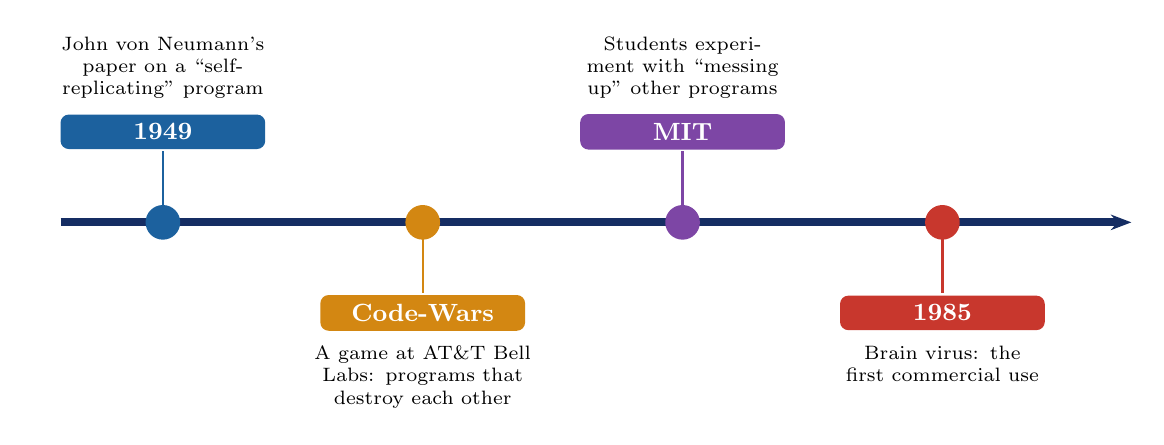
\begin{tikzpicture}
    \draw[navy,line width=3pt,->] (0,0) -- (13.6,0);
    \foreach \x/\c/\y/\t/\d in {
      1.3/ocean/1/1949/John von Neumann's paper on a ``self-replicating'' program,
      4.6/amber!90!black/-1/Code-Wars/A game at AT\&T Bell Labs: programs that destroy each other,
      7.9/grape/1/MIT/Students experiment with ``messing up'' other programs,
      11.2/brick/-1/1985/Brain virus: the first commercial use}
    {
      \fill[\c] (\x,0) circle (2.2mm);
      \draw[\c,thick] (\x,0) -- (\x,\y*0.9);
      \node[fill=\c,text=white,rounded corners=3pt,font=\small\bfseries,minimum width=26mm] at (\x,\y*1.15) {\t};
      \ifnum\y>0 \node[font=\scriptsize,text width=32mm,align=center,anchor=south] at (\x,1.45) {\d};\else \node[font=\scriptsize,text width=32mm,align=center,anchor=north] at (\x,-1.45) {\d};\fi
    }
  \end{tikzpicture}
  \vspace{4mm}
  \begin{block}{From idea to threat}
    \small The 1949 idea seemed impossible and was dropped. Code-Wars' authors \textbf{kept it secret} because they saw the danger. Harmless hobbies at Bell Labs and MIT gave rise to the \textbf{concept of computer viruses}.
  \end{block}
\end{frame}

% ------------------------------------------------------------
\begin{frame}{1985: The Brain (Pakistani) Virus}
  \begin{columns}[c]
    \begin{column}{0.5\textwidth}
      \centering
      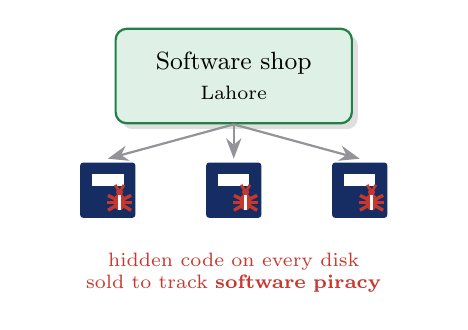
\begin{tikzpicture}
        \node[box=leaf,minimum width=30mm,minimum height=12mm] (shop) at (0,1.2) {Software shop\\\scriptsize Lahore};
        \foreach \x in {-1.6,0,1.6}{
          \fill[navy,rounded corners=1pt] (\x-0.35,-0.6) rectangle (\x+0.35,0.1);
          \fill[white] (\x-0.2,-0.05) rectangle (\x+0.2,-0.2);
          \pic[scale=0.35] at (\x+0.15,-0.4) {bug=brick};
          \draw[->,thick,ink!50] (shop.south) -- (\x,0.15);
        }
        \node[font=\scriptsize,text=brick,text width=50mm,align=center] at (0,-1.3) {hidden code on every disk sold to track \textbf{software piracy}};
      \end{tikzpicture}
    \end{column}
    \begin{column}{0.48\textwidth}
      \begin{itemize}\small\setlength{\itemsep}{4pt}
        \item Two Pakistani brothers wanted to \textbf{track piracy} of their low-cost software
        \item A small \textbf{self-replicating} snippet was hidden on nearly every disk
        \item It infected an \textbf{unauthorized user's} computer by disrupting operations
        \item Shows a popup: ``\textbf{Welcome to the Dungeon}''
      \end{itemize}
      \vspace{1mm}
      \begin{alertblock}{Lesson}
        \small Such programs multiplied so fast that today they are a threat to every computer.
      \end{alertblock}
    \end{column}
  \end{columns}
\end{frame}

% ------------------------------------------------------------
\begin{frame}{The Menace: Biological vs.\ Computer Virus}
  \centering
  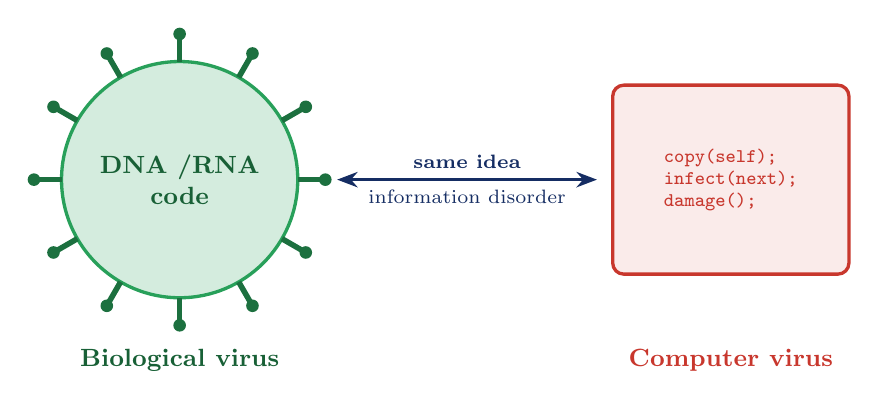
\begin{tikzpicture}
    \node[circle,fill=leaf!20,draw=leaf,very thick,minimum size=30mm] (b) at (0,0) {};
    \foreach \a in {0,30,...,330}{ \draw[leaf!70!black,line width=2pt] (\a:1.5) -- (\a:1.8); \fill[leaf!70!black] (\a:1.85) circle (0.08); }
    \node[font=\small\bfseries,text=leaf!60!black,align=center] at (0,0) {DNA \slash RNA\\code};
    \node[font=\small\bfseries,text=leaf!60!black] at (0,-2.3) {Biological virus};
    \node[draw=brick,fill=brick!10,very thick,rounded corners,minimum width=30mm,minimum height=24mm] (c) at (7,0) {};
    \node[font=\scriptsize\ttfamily,text=brick,align=left] at (7,0) {copy(self);\\infect(next);\\damage();};
    \node[font=\small\bfseries,text=brick] at (7,-2.3) {Computer virus};
    \draw[<->,very thick,navy] (2.0,0) -- node[above,font=\scriptsize\bfseries]{same idea} node[below,font=\scriptsize]{information disorder} (5.3,0);
  \end{tikzpicture}
  \vspace{3mm}
  \begin{block}{An information disorder}
    \small A biological virus takes over a living cell to make thousands of replicas. A computer virus carries \textbf{instructional code that makes copies of itself}, and spreads from machine to machine \textbf{like a forest fire}.
  \end{block}
\end{frame}

% ------------------------------------------------------------
\begin{frame}{The Damage Viruses Cause}
  \begin{columns}[T]
    \begin{column}{0.49\textwidth}
      \begin{alertblock}{Data loss}
        \small Apart from self-replication, the biggest devastation is \textbf{data loss}. Most viruses do this to perform even simple feats.
      \end{alertblock}
      \centering
      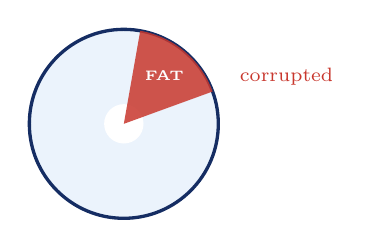
\begin{tikzpicture}
        \draw[navy,very thick,fill=sky] (0,0) circle (1.2);
        \fill[white] (0,0) circle (0.25);
        \fill[brick,opacity=0.85] (0,0) -- (20:1.2) arc (20:80:1.2) -- cycle;
        \node[font=\tiny\bfseries,text=white] at (50:0.8) {FAT};
        \node[font=\scriptsize,text=brick,anchor=west] at (1.35,0.6) {corrupted};
      \end{tikzpicture}
    \end{column}
    \begin{column}{0.49\textwidth}
      \textbf{Two common tricks}
      \begin{enumerate}\small\setlength{\itemsep}{4pt}
        \item Corrupt the most sensitive disk area: the \textbf{File Allocation Table (FAT)} or the directory area
        \item Modify the system's \textbf{interrupt organization}, so every read or write is routed through the virus code, causing interrupt clashes
      \end{enumerate}
      \vspace{2mm}
      \begin{block}{Even without a ``destroy'' instruction}
        \small A virus can still render a disk full of files \textbf{absolutely useless}.
      \end{block}
    \end{column}
  \end{columns}
\end{frame}

% ------------------------------------------------------------
\begin{frame}{The Process of Infection: Booting}
  \centering
  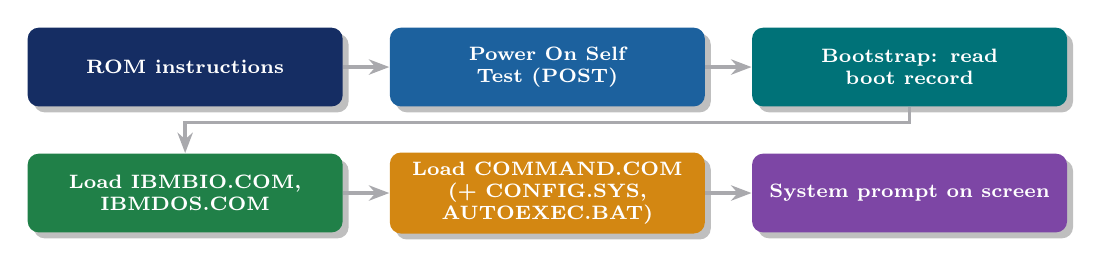
\begin{tikzpicture}
    \foreach \t/\c [count=\i from 0] in {ROM instructions/navy,Power On Self Test (POST)/ocean,Bootstrap: read boot record/aqua!80!black,Load IBMBIO.COM\comma{} IBMDOS.COM/leaf!80!black,Load COMMAND.COM (+ CONFIG.SYS\comma{} AUTOEXEC.BAT)/amber!90!black,System prompt on screen/grape}{
      \pgfmathsetmacro{\x}{mod(\i,3)*4.6}
      \pgfmathsetmacro{\y}{-floor(\i/3)*1.6}
      \node[fill=\c,text=white,font=\scriptsize\bfseries,rounded corners=4pt,minimum width=40mm,text width=37mm,align=center,minimum height=10mm,drop shadow] (s\i) at (\x,\y) {\t};
    }
    \draw[flow=ink!40] (s0) -- (s1); \draw[flow=ink!40] (s1) -- (s2);
    \draw[flow=ink!40] (s2.south) -- ++(0,-0.2) -| (s3.north);
    \draw[flow=ink!40] (s3) -- (s4); \draw[flow=ink!40] (s4) -- (s5);
  \end{tikzpicture}
  \vspace{4mm}
  \begin{alertblock}{Where infection begins}
    \small As soon as a computer \textbf{boots from a contaminated disk} or \textbf{executes an infected program}, whatever viruses are present are activated and begin to spread throughout the system.
  \end{alertblock}
\end{frame}

% ------------------------------------------------------------
\begin{frame}{The Interrupt Mechanism and ISRs}
  \centering
  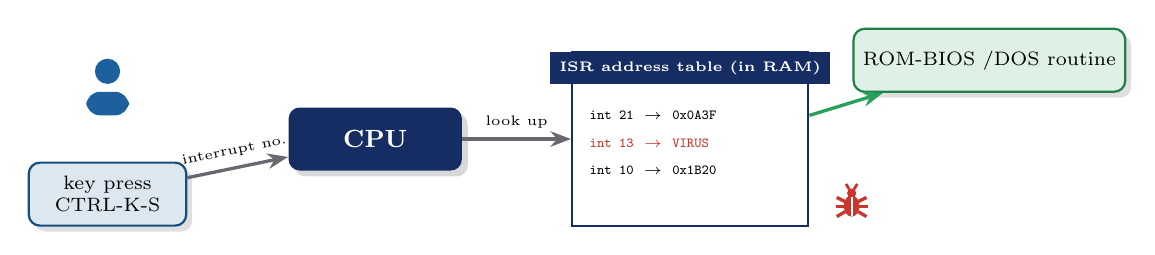
\begin{tikzpicture}
    \pic[scale=1] at (0,0) {person=ocean};
    \node[box=ocean,minimum width=20mm,font=\scriptsize] (k) at (0,-1.1) {key press\\CTRL-K-S};
    \node[solid box=navy,minimum width=22mm] (cpu) at (3.4,-0.4) {CPU};
    \draw[flow] (k) -- node[above,font=\tiny,sloped]{interrupt no.} (cpu);
    \node[draw=navy,thick,fill=white,minimum width=30mm,minimum height=22mm] (tab) at (7.4,-0.4) {};
    \node[fill=navy,text=white,font=\tiny\bfseries,minimum width=30mm,anchor=north] at (tab.north) {ISR address table (in RAM)};
    \node[font=\tiny\ttfamily,anchor=west] at (6.0,-0.1) {int 21 \,$\to$\, 0x0A3F};
    \node[font=\tiny\ttfamily,anchor=west,text=brick] at (6.0,-0.45) {int 13 \,$\to$\, \textbf{VIRUS}};
    \node[font=\tiny\ttfamily,anchor=west] at (6.0,-0.8) {int 10 \,$\to$\, 0x1B20};
    \draw[flow] (cpu) -- node[above,font=\tiny]{look up} (tab);
    \pic[scale=0.45] at (9.45,-1.25) {bug=brick};
    \node[box=leaf,minimum width=24mm,font=\scriptsize] (isr) at (11.2,0.6) {ROM-BIOS \slash DOS routine};
    \draw[flow=leaf] ([yshift=3mm]tab.east) -- (isr);
  \end{tikzpicture}
  \vspace{3mm}
  \begin{itemize}\small
    \item All I/O on a PC is done by \textbf{interrupts}; routines that serve them are \textbf{Interrupt Service Routines (ISRs)}
    \item The CPU looks up the interrupt number in a \textbf{table} to find the routine, runs it, and returns control
    \item The table sits in \textbf{RAM}, so user programs can change it, and that is exactly \textbf{what a virus does}
  \end{itemize}
\end{frame}

% ------------------------------------------------------------
\begin{frame}{Classification of Viruses}
  \centering
  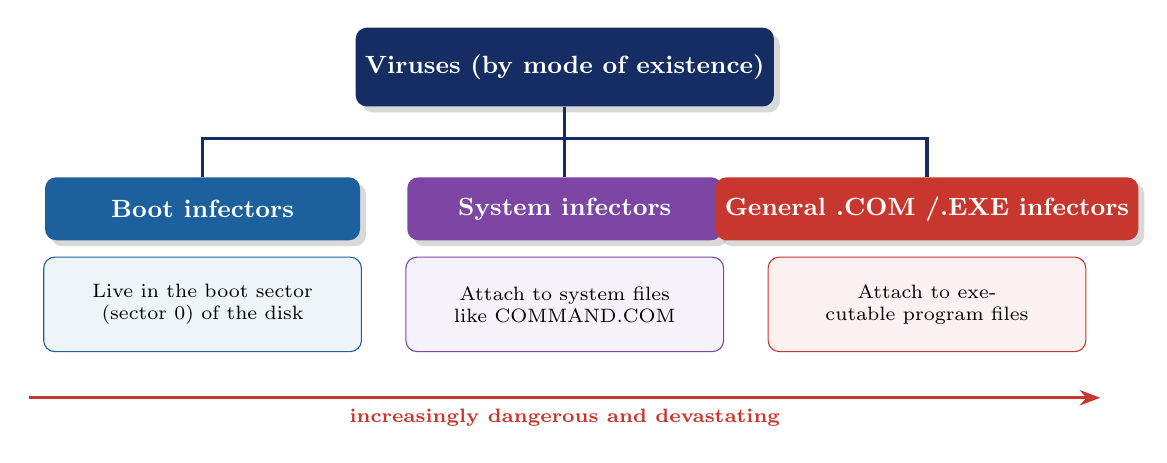
\begin{tikzpicture}
    \node[solid box=navy,minimum width=48mm,minimum height=10mm] (t) at (0,0) {Viruses (by mode of existence)};
    \foreach \t/\c/\x/\d [count=\i] in {
      Boot infectors/ocean/-4.6/Live in the boot sector (sector 0) of the disk,
      System infectors/grape/0/Attach to system files like COMMAND.COM,
      General .COM \slash .EXE infectors/brick/4.6/Attach to executable program files}
    {
      \node[solid box=\c,minimum width=40mm] (n\i) at (\x,-1.8) {\t};
      \draw[navy,very thick] (t.south) -- ++(0,-0.4) -| (n\i.north);
      \node[draw=\c,fill=\c!7,rounded corners,text width=38mm,minimum height=12mm,align=center,font=\scriptsize,anchor=north] at ([yshift=-2mm]n\i.south) {\d};
    }
    \draw[->,very thick,brick] (-6.8,-4.2) -- node[below,font=\scriptsize\bfseries,text=brick]{increasingly dangerous and devastating} (6.8,-4.2);
  \end{tikzpicture}
\end{frame}

% ------------------------------------------------------------
\begin{frame}{Boot Infectors}
  \begin{columns}[c]
    \begin{column}{0.48\textwidth}
      \centering
      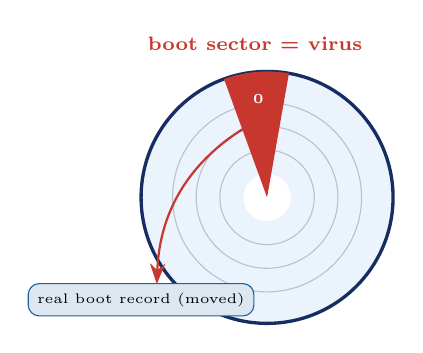
\begin{tikzpicture}
        \draw[navy,very thick,fill=sky] (0,0) circle (1.6);
        \fill[white] (0,0) circle (0.3);
        \foreach \r in {0.6,0.9,1.2} \draw[navy!30] (0,0) circle (\r);
        \fill[brick] (0,0) -- (80:1.6) arc (80:110:1.6) -- cycle;
        \node[font=\tiny\bfseries,text=white] at (95:1.25) {0};
        \node[font=\scriptsize\bfseries,text=brick,anchor=south] at (95:1.75) {boot sector = virus};
        \node[fill=ocean!15,draw=ocean,font=\tiny,rounded corners] at (-1.6,-1.3) {real boot record (moved)};
        \draw[->,brick,thick] (95:1.0) to[bend right=30] (-1.4,-1.1);
      \end{tikzpicture}
    \end{column}
    \begin{column}{0.5\textwidth}
      \begin{itemize}\small\setlength{\itemsep}{3pt}
        \item Physically reside in the \textbf{boot sector [0]} of the disk, not in a program file
        \item Load right after POST and stay in control \textbf{at all times}
        \item Can trap soft booting (CTRL+ALT+DEL) and \textbf{infect a clean floppy}
        \item Move the real boot record elsewhere, and pass control to it after loading, otherwise the disk would not work
        \item Typically create \textbf{``bad sectors''}; stay in memory until shutdown and disk reformat
      \end{itemize}
    \end{column}
  \end{columns}
\end{frame}

% ------------------------------------------------------------
\begin{frame}{System Infectors}
  \begin{columns}[c]
    \begin{column}{0.48\textwidth}
      \centering
      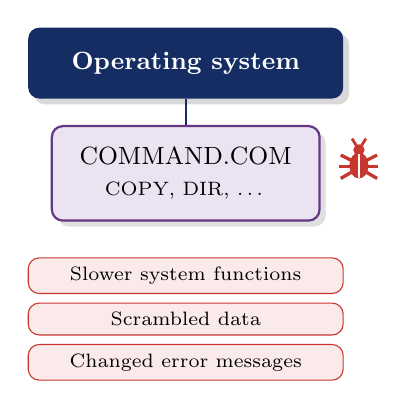
\begin{tikzpicture}
        \node[solid box=navy,minimum width=40mm,minimum height=9mm] (os) at (0,1.4) {Operating system};
        \node[box=grape,minimum width=34mm,minimum height=12mm] (cc) at (0,0) {COMMAND.COM\\\scriptsize COPY, DIR, \dots};
        \pic[scale=0.55] at (2.2,0.1) {bug=brick};
        \draw[navy,thick] (os) -- (cc);
        \foreach \t/\y in {Slower system functions/-1.3,Scrambled data/-1.85,Changed error messages/-2.4}
          \node[fill=brick!10,draw=brick,rounded corners,font=\scriptsize,minimum width=40mm] at (0,\y) {\t};
      \end{tikzpicture}
    \end{column}
    \begin{column}{0.5\textwidth}
      \begin{itemize}\small\setlength{\itemsep}{3pt}
        \item Infect the \textbf{components of the system itself}
        \item In MS-DOS, \textbf{COMMAND.COM} holds the internal commands (COPY, DIR, \dots); without it they cannot load
        \item Attach to COMMAND.COM or other memory-resident files and \textbf{manipulate} them
      \end{itemize}
      \begin{block}{Differ from boot infectors}
        \small They gain control \textbf{after} booting, and infect disks that contain the system files only. They may act after some time, or begin subtle changes at once.
      \end{block}
    \end{column}
  \end{columns}
\end{frame}

% ------------------------------------------------------------
\begin{frame}{General .COM and .EXE Infectors}
  \centering
  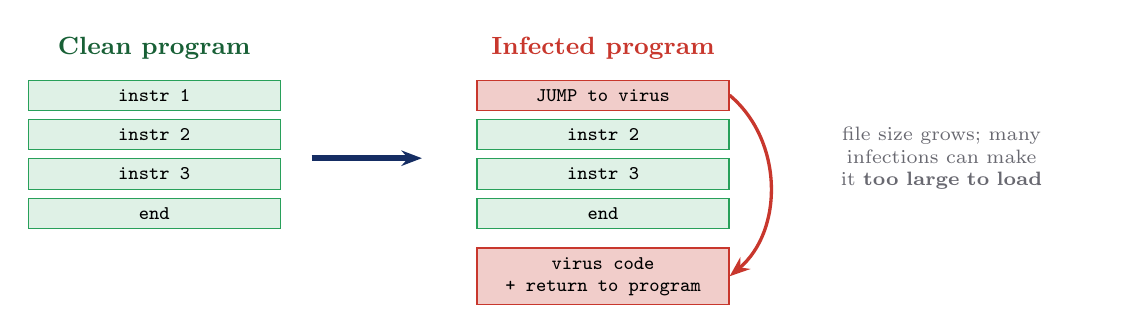
\begin{tikzpicture}
    \node[font=\small\bfseries,text=leaf!60!black] at (1.6,1.3) {Clean program};
    \foreach \t [count=\i from 0] in {instr 1,instr 2,instr 3,end}
      \node[fill=leaf!15,draw=leaf,font=\scriptsize\ttfamily,minimum width=32mm] at (1.6,0.7-\i*0.5) {\t};
    \draw[flow=navy,line width=2pt] (3.6,-0.1) -- (5.0,-0.1);
    \node[font=\small\bfseries,text=brick] at (7.3,1.3) {Infected program};
    \node[fill=brick!25,draw=brick,font=\scriptsize\ttfamily,minimum width=32mm] (j) at (7.3,0.7) {JUMP to virus};
    \foreach \t [count=\i from 1] in {instr 2,instr 3,end}
      \node[fill=leaf!15,draw=leaf,font=\scriptsize\ttfamily,minimum width=32mm] at (7.3,0.7-\i*0.5) {\t};
    \node[fill=brick!25,draw=brick,font=\scriptsize\ttfamily,minimum width=32mm,align=center] (v) at (7.3,-1.6) {virus code\\+ return to program};
    \draw[->,brick,very thick] (j.east) to[bend left=50] (v.east);
    \node[font=\scriptsize,text=ink!70,text width=36mm,align=center] at (11.6,-0.1) {file size grows; many infections can make it \textbf{too large to load}};
  \end{tikzpicture}
  \vspace{2mm}
  \begin{itemize}\small
    \item \textbf{Most dangerous} of the three classes: they can spread to almost any executable program
    \item Change the program's instructions into a \textbf{jump} to the virus, which runs first and then lets the program continue
    \item Stay \textbf{memory resident} and infect every program loaded after them
  \end{itemize}
\end{frame}

% ------------------------------------------------------------
\begin{frame}{The Three Classes Side by Side}
  \centering
  \renewcommand{\arraystretch}{1.5}
  \small
  \begin{tabular}{>{\bfseries}l >{\columncolor{ocean!8}}p{3.6cm} >{\columncolor{grape!8}}p{3.6cm} >{\columncolor{brick!8}}p{3.6cm}}
    \toprule
    \rowcolor{navy}\textcolor{white}{Feature} & \textcolor{white}{\textbf{Boot infector}} & \textcolor{white}{\textbf{System infector}} & \textcolor{white}{\textbf{.COM \slash .EXE infector}}\\
    \midrule
    Lives in & Boot sector (0) & COMMAND.COM, system files & Any executable file\\
    Gets control & Right after POST & After booting & When the program runs\\
    Typical sign & Bad sectors & Slow or odd system behaviour & Larger file sizes\\
    Danger & High & High & \textbf{Highest}\\
    \bottomrule
  \end{tabular}
\end{frame}

% ------------------------------------------------------------
\begin{frame}{Famous Viruses (1): Scores, Brain, Lehigh}
  \centering
  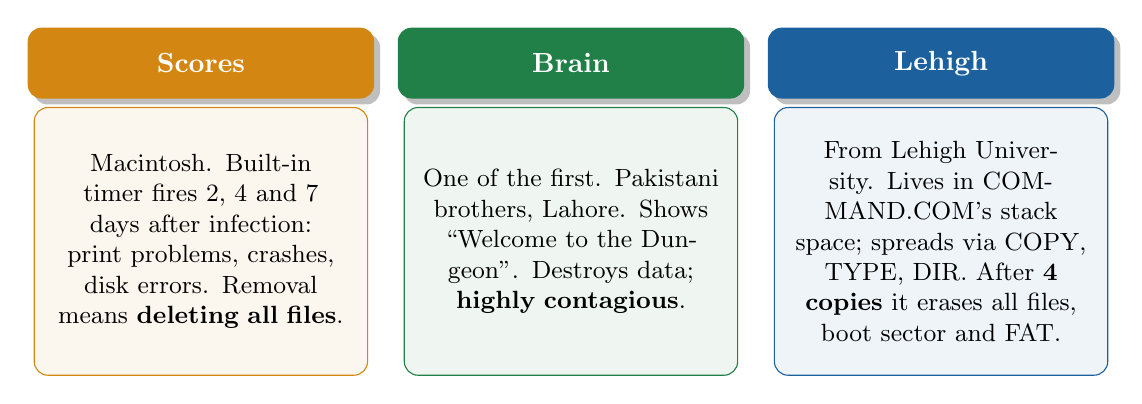
\begin{tikzpicture}
    \foreach \x/\c/\t/\d in {
      0/amber!90!black/Scores/Macintosh. Built-in timer fires 2\comma{} 4 and 7 days after infection: print problems\comma{} crashes\comma{} disk errors. Removal means \textbf{deleting all files}.,
      4.7/leaf!80!black/Brain/One of the first. Pakistani brothers\comma{} Lahore. Shows ``Welcome to the Dungeon''. Destroys data; \textbf{highly contagious}.,
      9.4/ocean/Lehigh/From Lehigh University. Lives in COMMAND.COM's stack space; spreads via COPY\comma{} TYPE\comma{} DIR. After \textbf{4 copies} it erases all files\comma{} boot sector and FAT.}
    {
      \node[fill=\c,text=white,rounded corners=5pt,font=\bfseries,minimum width=44mm,minimum height=9mm,drop shadow] (h) at (\x,0) {\t};
      \node[draw=\c,fill=\c!7,rounded corners=5pt,text width=40mm,minimum height=34mm,font=\small,anchor=north,align=center] at ([yshift=-1mm]h.south) {\d};
    }
  \end{tikzpicture}
\end{frame}

% ------------------------------------------------------------
\begin{frame}{Famous Viruses (2): Friday the 13th}
  \begin{columns}[c]
    \begin{column}{0.44\textwidth}
      \centering
      
\begin{tikzpicture}
        \draw[brick,very thick,fill=white,rounded corners=4pt] (0,0) rectangle (3,3);
        \fill[brick,rounded corners=4pt] (0,2.2) rectangle (3,3);
        \fill[brick] (0,2.2) rectangle (3,2.5);
        \node[white,font=\small\bfseries] at (1.5,2.6) {FRIDAY};
        \node[brick,font=\fontsize{40}{44}\selectfont\bfseries] at (1.5,1.05) {13};
        \foreach \x in {0.6,2.4} \fill[navy] (\x,3) circle (0.12);
        \node[font=\scriptsize\bfseries,text=brick] at (1.5,-0.4) {all files deleted};
      \end{tikzpicture}
    \end{column}
    \begin{column}{0.54\textwidth}
      \begin{itemize}\small\setlength{\itemsep}{3pt}
        \item Attacks COMMAND.COM \textbf{and} other executable files
        \item When the first .COM or .EXE runs, it captures an interrupt and inserts its own code
        \item In .EXE files the code goes at the \textbf{end}: the file grows by \textbf{1808 bytes} each time
        \item In .COM files it goes at the \textbf{beginning}
        \item Programs become too large to load, and later run much \textbf{slower}
      \end{itemize}
      \begin{alertblock}{The worst disaster}
        \small If an infected program runs when the system date is \textbf{Friday the 13th}, all files get deleted.
      \end{alertblock}
    \end{column}
  \end{columns}
\end{frame}

% ------------------------------------------------------------
\begin{frame}{Famous Viruses (3): Slug, Raindrops, Happy Birthday}
  \centering
  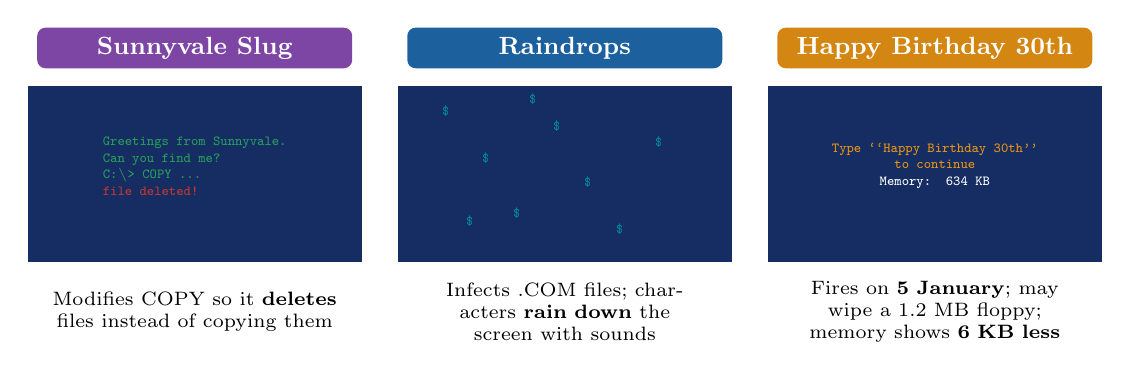
\begin{tikzpicture}
    % screen 1
    \foreach \x/\c/\t in {0/grape/Sunnyvale Slug,4.7/ocean/Raindrops,9.4/amber!90!black/Happy Birthday 30th}{
      \draw[navy,very thick,fill=navy] (\x-2.1,-0.2) rectangle (\x+2.1,2.0);
      \node[fill=\c,text=white,rounded corners=3pt,font=\small\bfseries,minimum width=40mm] at (\x,2.5) {\t};
    }
    \node[font=\tiny\ttfamily,text=leaf,align=left] at (0,1.0) {Greetings from Sunnyvale.\\Can you find me?\\C:\textbackslash> COPY \dots\\\textcolor{brick}{file deleted!}};
    \foreach \x/\y in {3.2/1.7,3.7/1.1,4.1/0.4,4.6/1.5,5.0/0.8,5.4/0.2,5.9/1.3,4.3/1.85,3.5/0.3}
      \node[font=\tiny\ttfamily,text=aqua] at (\x,\y) {\$};
    \node[font=\tiny\ttfamily,text=amber,align=center] at (9.4,1.0) {Type ``Happy Birthday 30th''\\to continue\\\textcolor{white}{Memory: 634 KB}};
    \node[font=\scriptsize,text width=40mm,align=center] at (0,-0.85) {Modifies COPY so it \textbf{deletes} files instead of copying them};
    \node[font=\scriptsize,text width=40mm,align=center] at (4.7,-0.85) {Infects .COM files; characters \textbf{rain down} the screen with sounds};
    \node[font=\scriptsize,text width=40mm,align=center] at (9.4,-0.85) {Fires on \textbf{5 January}; may wipe a 1.2 MB floppy; memory shows \textbf{6 KB less}};
  \end{tikzpicture}
\end{frame}

% ------------------------------------------------------------
\begin{frame}{A Rogues' Gallery of Viruses}
  \centering
  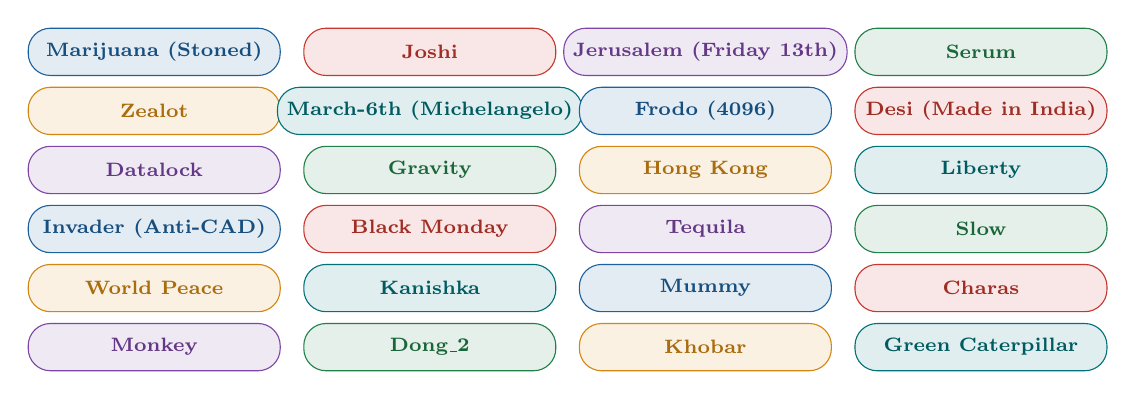
\begin{tikzpicture}
    \foreach \t [count=\i from 0] in {Marijuana (Stoned),Joshi,Jerusalem (Friday 13th),Serum,Zealot,March-6th (Michelangelo),Frodo (4096),Desi (Made in India),Datalock,Gravity,Hong Kong,Liberty,Invader (Anti-CAD),Black Monday,Tequila,Slow,World Peace,Kanishka,Mummy,Charas,Monkey,Dong\_2,Khobar,Green Caterpillar}{
      \pgfmathsetmacro{\x}{mod(\i,4)*3.5}
      \pgfmathsetmacro{\y}{-floor(\i/4)*0.75}
      \pgfmathtruncatemacro{\k}{mod(\i,6)}
      \ifcase\k \def\cc{ocean}\or \def\cc{brick}\or \def\cc{grape}\or \def\cc{leaf!80!black}\or \def\cc{amber!90!black}\else \def\cc{aqua!80!black}\fi
      \node[fill=\cc!12,draw=\cc,rounded corners=8pt,font=\scriptsize\bfseries,text=\cc!80!black,minimum width=32mm,minimum height=6mm] at (\x,\y) {\t};
    }
  \end{tikzpicture}
  \vspace{3mm}

  {\small A comprehensive list cannot be built, because \textbf{every other day a new virus} joins it.}
\end{frame}

% ------------------------------------------------------------
\begin{frame}{The Four Phases of a Virus (Fig.\ 6.2)}
  \begin{columns}[c]
    \begin{column}{0.4\textwidth}
      \centering
      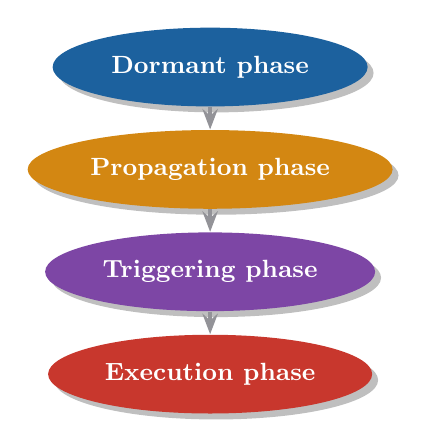
\begin{tikzpicture}
        \foreach \t/\c [count=\i from 0] in {Dormant phase/ocean,Propagation phase/amber!90!black,Triggering phase/grape,Execution phase/brick}{
          \node[ellipse,fill=\c,text=white,font=\small\bfseries,minimum width=40mm,minimum height=10mm,drop shadow] (p\i) at (0,-\i*1.3) {\t};
        }
        \foreach \i [evaluate=\i as \j using int(\i+1)] in {0,1,2} \draw[flow=ink!50] (p\i) -- (p\j);
      \end{tikzpicture}
    \end{column}
    \begin{column}{0.58\textwidth}
      \begin{description}\small\setlength{\itemsep}{4pt}
        \item[\textcolor{ocean}{Dormant}] The virus is \textbf{idle}, waiting for a date or event. Not all viruses have this stage.
        \item[\textcolor{amber!80!black}{Propagation}] The ``spread over'' phase: the virus places \textbf{replicas} of itself; each infected program holds a clone.
        \item[\textcolor{grape}{Triggering}] The virus is \textbf{activated} to do the task it was created for.
        \item[\textcolor{brick}{Execution}] The \textbf{actual function} is performed: harmless or damaging.
      \end{description}
    \end{column}
  \end{columns}
\end{frame}

% ------------------------------------------------------------
\begin{frame}{Prevention Is Better Than Cure}
  \begin{columns}[c]
    \begin{column}{0.4\textwidth}
      \centering
      
\begin{tikzpicture}
        \fill[leaf!15,draw=leaf,very thick] (0,1.6) -- (1.4,1.1) -- (1.25,-0.5) -- (0,-1.5) -- (-1.25,-0.5) -- (-1.4,1.1) -- cycle;
        \node[font=\Huge\bfseries,text=leaf!70!black] at (0,0.2) {\checkmark};
        \node[font=\scriptsize\bfseries,text=leaf!60!black,text width=40mm,align=center] at (0,-2.0) {Viruses are made \textbf{faster} than the vaccines};
      \end{tikzpicture}
    \end{column}
    \begin{column}{0.58\textwidth}
      \textbf{Simple precautionary measures}
      \begin{itemize}\small\setlength{\itemsep}{2pt}
        \item Add \textbf{CHKDSK} to AUTOEXEC.BAT; investigate if hidden files increase
        \item \textbf{Stop} using pirated software
        \item Use \textbf{write-protect tags} on original diskettes
        \item Keep a proper \textbf{backup} of all data and programs
        \item Copy files carefully: put COPY in a batch file with CHKDSK
        \item \textbf{Reformat} used floppies
        \item Do not let \textbf{unauthorized users} use the system
        \item \textbf{Restrict} outside floppies
      \end{itemize}
    \end{column}
  \end{columns}
\end{frame}

% ------------------------------------------------------------
\begin{frame}{The Cure: What Anti-Viral Programs Do}
  \begin{columns}[c]
    \begin{column}{0.52\textwidth}
      \centering
      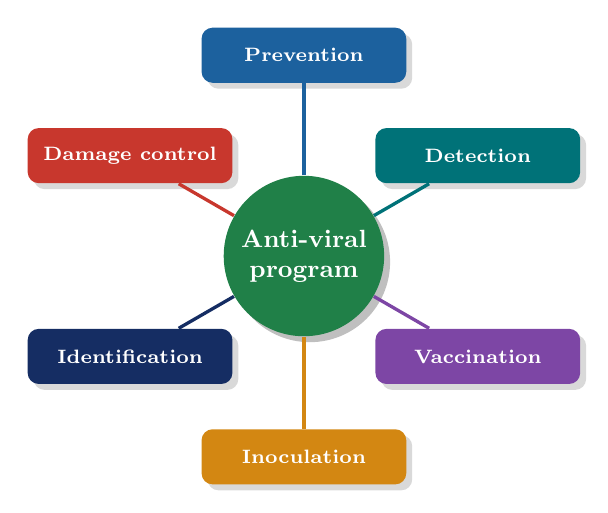
\begin{tikzpicture}
        \node[circle,fill=leaf!80!black,text=white,font=\small\bfseries,minimum size=20mm,align=center,drop shadow] (c) at (0,0) {Anti-viral\\program};
        \foreach \a/\t/\c in {90/Prevention/ocean,30/Detection/aqua!80!black,-30/Vaccination/grape,-90/Inoculation/amber!90!black,-150/Identification/navy,150/Damage control/brick}{
          \node[solid box=\c,minimum width=26mm,minimum height=7mm,font=\scriptsize\bfseries] (s\a) at (\a:2.55) {\t};
          \draw[\c,very thick] (c) -- (s\a);
        }
      \end{tikzpicture}
    \end{column}
    \begin{column}{0.46\textwidth}
      \begin{block}{Viruses are not omnipotent}
        \small They can be cured with anti-viral programs that perform one or more of these six functions.
      \end{block}
      \vspace{2mm}
      \begin{exampleblock}{A good anti-viral utility}
        \small Checks whether the system is infected, \textbf{stops} viruses from infecting it, and does \textbf{not allow modification} of executable files.
      \end{exampleblock}
    \end{column}
  \end{columns}
\end{frame}

% ------------------------------------------------------------
\begin{frame}{Preventers, Detectors and Identifiers}
  \centering
  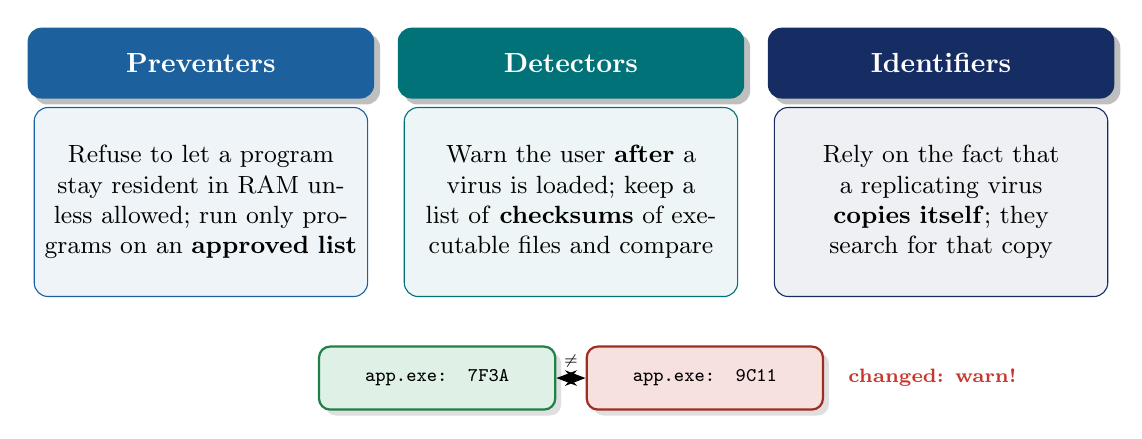
\begin{tikzpicture}
    \foreach \x/\c/\t/\d in {
      0/ocean/Preventers/Refuse to let a program stay resident in RAM unless allowed; run only programs on an \textbf{approved list},
      4.7/aqua!80!black/Detectors/Warn the user \textbf{after} a virus is loaded; keep a list of \textbf{checksums} of executable files and compare,
      9.4/navy/Identifiers/Rely on the fact that a replicating virus \textbf{copies itself}; they search for that copy}
    {
      \node[fill=\c,text=white,rounded corners=5pt,font=\bfseries,minimum width=44mm,minimum height=9mm,drop shadow] (h) at (\x,0) {\t};
      \node[draw=\c,fill=\c!7,rounded corners=5pt,text width=40mm,minimum height=24mm,font=\small,anchor=north,align=center] at ([yshift=-1mm]h.south) {\d};
    }
    % checksum mini diagram
    \node[box=leaf,font=\scriptsize\ttfamily,minimum width=30mm] (a) at (3.0,-4.0) {app.exe: 7F3A};
    \node[box=brick,font=\scriptsize\ttfamily,minimum width=30mm] (b) at (6.4,-4.0) {app.exe: 9C11};
    \draw[<->,very thick] (a) -- node[above,font=\tiny]{$\neq$} (b);
    \node[font=\scriptsize\bfseries,text=brick,anchor=west] at (8.1,-4.0) {changed: warn!};
  \end{tikzpicture}
\end{frame}

% ------------------------------------------------------------
\begin{frame}{Vaccinators and Inoculators}
  \begin{columns}[T]
    \begin{column}{0.49\textwidth}
      \centering\textbf{\textcolor{grape}{Vaccinators}}\\[2mm]
      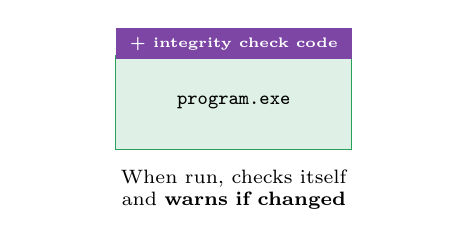
\begin{tikzpicture}
        \node[fill=leaf!15,draw=leaf,font=\scriptsize\ttfamily,minimum width=30mm,minimum height=12mm] (f) at (0,0) {program.exe};
        \node[fill=grape,text=white,font=\tiny\bfseries,minimum width=30mm] at (0,0.75) {+ integrity check code};
        \node[font=\scriptsize,text width=50mm,align=center] at (0,-1.1) {When run, checks itself and \textbf{warns if changed}};
      \end{tikzpicture}\\[1mm]
      {\small Inject some code into executable files. The injected code performs an \textbf{integrity check} on the program being executed.}
    \end{column}
    \begin{column}{0.49\textwidth}
      \centering\textbf{\textcolor{amber!80!black}{Inoculators}}\\[2mm]
      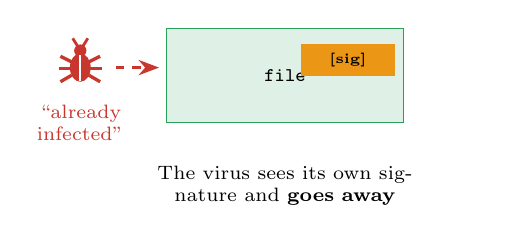
\begin{tikzpicture}
        \node[fill=leaf!15,draw=leaf,font=\scriptsize\ttfamily,minimum width=30mm,minimum height=12mm] (f) at (0,0) {file};
        \node[fill=amber,font=\tiny\bfseries,minimum width=12mm] at (0.8,0.2) {[sig]};
        \pic[scale=0.6] at (-2.6,0.1) {bug=brick};
        \node[font=\scriptsize,text=brick,align=center] at (-2.6,-0.6) {``already\\infected''};
        \draw[->,brick,thick,dashed] (-2.15,0.1) -- (-1.6,0.1);
        \node[font=\scriptsize,text width=50mm,align=center] at (0,-1.4) {The virus sees its own signature and \textbf{goes away}};
      \end{tikzpicture}\\[1mm]
      {\small Insert the \textbf{virus signature} into files and areas, so the virus believes they are already infected.}
    \end{column}
  \end{columns}
\end{frame}

% ------------------------------------------------------------
\begin{frame}{Damage Control and the Hard Truth}
  \begin{columns}[T]
    \begin{column}{0.49\textwidth}
      \begin{block}{Damage control}
        \small
        \textbf{Preventive:} stop direct access attempts such as formatting and deleting; write-protect the hard disk while testing unfamiliar software.\\[3pt]
        \textbf{Restorative:} keep a copy of the CMOS information, boot sector and FAT in a safe place, like a floppy.
      \end{block}
    \end{column}
    \begin{column}{0.49\textwidth}
      \begin{alertblock}{No 100\% foolproof anti-virus}
        \small
        \begin{itemize}\setlength{\itemsep}{2pt}
          \item A virus can hide in many ways
          \item Virus writers keep \textbf{altering} their code to avoid detection
          \item So there is no perfect anti-virus, and in principle \textbf{there never will be}
        \end{itemize}
      \end{alertblock}
    \end{column}
  \end{columns}
  \vspace{3mm}
  \centering
  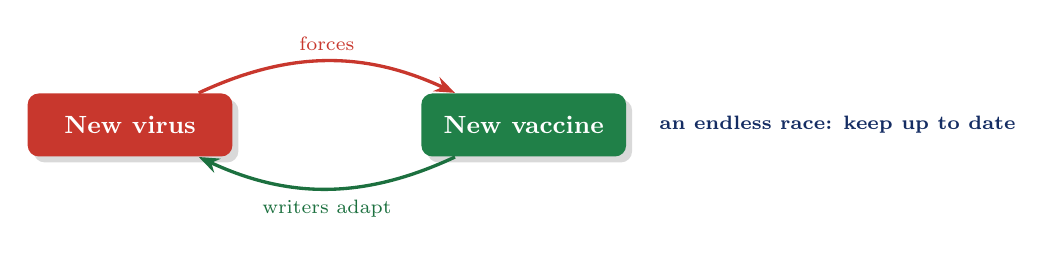
\begin{tikzpicture}
    \node[solid box=brick,minimum width=26mm] (v) at (0,0) {New virus};
    \node[solid box=leaf!80!black,minimum width=26mm] (a) at (5,0) {New vaccine};
    \draw[->,very thick,brick] (v) to[bend left=25] node[above,font=\scriptsize]{forces} (a);
    \draw[->,very thick,leaf!70!black] (a) to[bend left=25] node[below,font=\scriptsize]{writers adapt} (v);
    \node[font=\scriptsize\bfseries,text=navy,anchor=west] at (6.6,0) {an endless race: keep up to date};
  \end{tikzpicture}
\end{frame}

% ------------------------------------------------------------
\begin{frame}{Hardening: The Guest Account Problem}
  \begin{columns}[c]
    \begin{column}{0.48\textwidth}
      \centering
      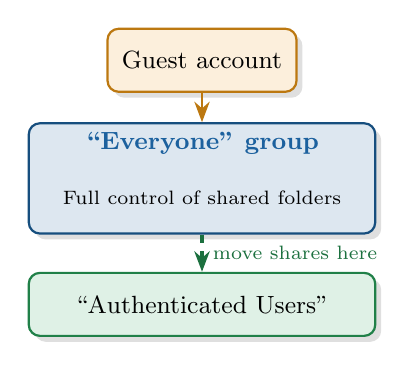
\begin{tikzpicture}
        \node[box=amber,minimum width=24mm] (g) at (0,1.5) {Guest account};
        \node[box=ocean,minimum width=44mm,minimum height=14mm] (e) at (0,0) {};
        \node[font=\small\bfseries,text=ocean,anchor=north] at (e.north) {``Everyone'' group};
        \node[font=\scriptsize] at (0,-0.25) {Full control of shared folders};
        \draw[->,thick,amber!80!black] (g) -- (e);
        \node[box=leaf,minimum width=44mm] (au) at (0,-1.6) {``Authenticated Users''};
        \draw[->,very thick,leaf!70!black,dashed] (e) -- node[right,font=\scriptsize]{move shares here} (au);
      \end{tikzpicture}
    \end{column}
    \begin{column}{0.5\textwidth}
      \begin{itemize}\small\setlength{\itemsep}{4pt}
        \item In Windows 2000 the Guest account is \textbf{disabled by default}; enabling it allows \textbf{anonymous} access
        \item A shared folder's default permission is: \textbf{Everyone has full control}
        \item Guest is part of ``Everyone'', so security is \textbf{compromised}
      \end{itemize}
      \begin{exampleblock}{Standard practice}
        \small Remove share permissions from ``Everyone'' and give them to ``Authenticated Users''.
      \end{exampleblock}
    \end{column}
  \end{columns}
\end{frame}

% ------------------------------------------------------------
\begin{frame}{Steps to Configure the Guest Account}
  \centering
  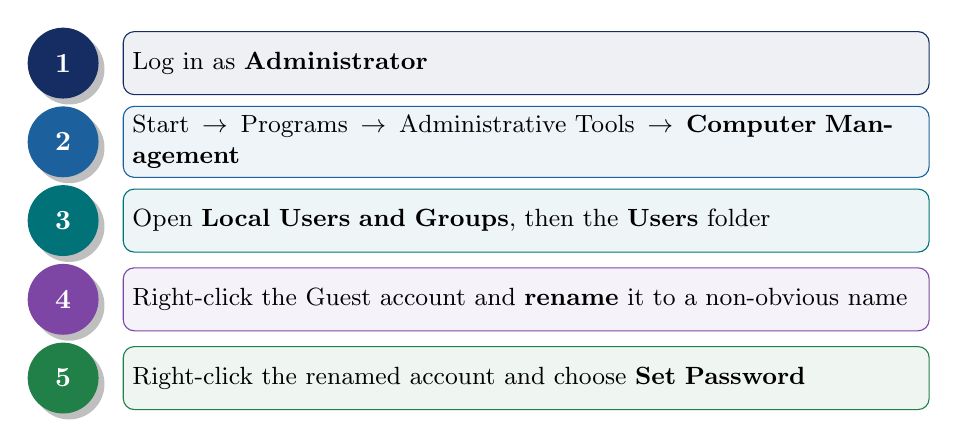
\begin{tikzpicture}
    \foreach \t/\c [count=\i] in {
      Log in as \textbf{Administrator}/navy,
      Start \,$\rightarrow$\, Programs \,$\rightarrow$\, Administrative Tools \,$\rightarrow$\, \textbf{Computer Management}/ocean,
      Open \textbf{Local Users and Groups}\comma{} then the \textbf{Users} folder/aqua!80!black,
      Right-click the Guest account and \textbf{rename} it to a non-obvious name/grape,
      Right-click the renamed account and choose \textbf{Set Password}/leaf!80!black}
    {
      \node[circle,fill=\c,text=white,font=\bfseries,minimum size=9mm,drop shadow] (c\i) at (0,-\i*1.0) {\i};
      \node[draw=\c,fill=\c!7,rounded corners=4pt,anchor=west,text width=100mm,minimum height=8mm,font=\small] at ([xshift=3mm]c\i.east) {\t};
    }
  \end{tikzpicture}
  \vspace{2mm}

  {\small A renamed, password-protected account gives attackers \textbf{nothing obvious to guess}.}
\end{frame}

% ------------------------------------------------------------
\begin{frame}{Hardening Network Activity}
  \centering
  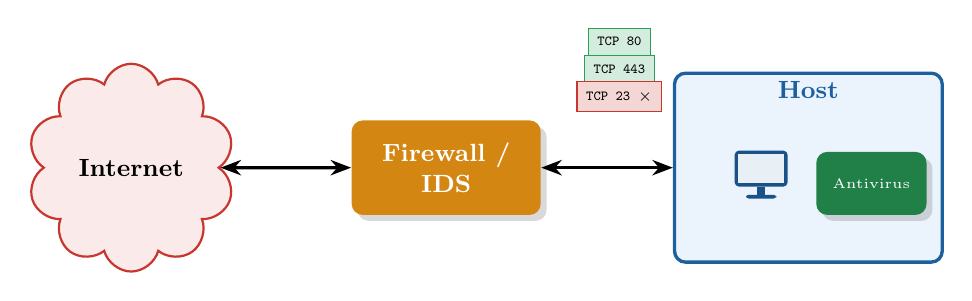
\begin{tikzpicture}
    \node[cloud,cloud puffs=10,draw=brick,fill=brick!10,thick,minimum width=2.4cm,minimum height=1.5cm,font=\small\bfseries] (net) at (0,0) {Internet};
    \node[solid box=amber!90!black,minimum width=24mm,minimum height=12mm] (fw) at (4.0,0) {Firewall \slash\\IDS};
    \node[draw=ocean,very thick,fill=sky,rounded corners,minimum width=34mm,minimum height=24mm] (host) at (8.6,0) {};
    \node[font=\small\bfseries,text=ocean,anchor=north] at (host.north) {Host};
    \pic[scale=0.8] at (8.0,-0.2) {pc=ocean};
    \node[solid box=leaf!80!black,minimum width=14mm,font=\tiny] at (9.4,-0.2) {Antivirus};
    \draw[<->,very thick] (net) -- (fw); \draw[<->,very thick] (fw) -- (host);
    \foreach \p/\ok/\y in {TCP 80/1/1.6,TCP 443/1/1.25,TCP 23/0/0.9}{
      \ifnum\ok=1 \node[fill=leaf!20,draw=leaf,font=\tiny\ttfamily] at (6.2,\y) {\p\ \checkmark};
      \else \node[fill=brick!20,draw=brick,font=\tiny\ttfamily] at (6.2,\y) {\p\ $\times$}; \fi
    }
  \end{tikzpicture}
  \vspace{3mm}
  \begin{block}{Next step after accounts}
    \small Install a \textbf{host-based antivirus} and a \textbf{firewall\slash intrusion detection system}. Configure which \textbf{TCP\slash UDP ports} can be accessed, so undesired communication does not happen on any port.
  \end{block}
\end{frame}

% ------------------------------------------------------------
\begin{frame}{Six Types of Malicious Code}
  \centering
  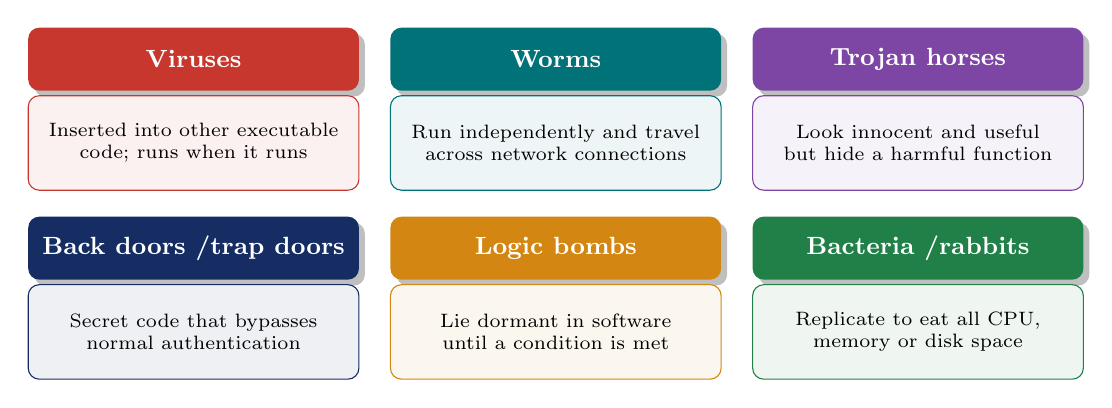
\begin{tikzpicture}
    \foreach \t/\d/\c [count=\i from 0] in {
      Viruses/Inserted into other executable code; runs when it runs/brick,
      Worms/Run independently and travel across network connections/aqua!80!black,
      Trojan horses/Look innocent and useful but hide a harmful function/grape,
      Back doors \slash trap doors/Secret code that bypasses normal authentication/navy,
      Logic bombs/Lie dormant in software until a condition is met/amber!90!black,
      Bacteria \slash rabbits/Replicate to eat all CPU\comma{} memory or disk space/leaf!80!black}
    {
      \pgfmathsetmacro{\x}{mod(\i,3)*4.6}
      \pgfmathsetmacro{\y}{-floor(\i/3)*2.4}
      \node[fill=\c,text=white,font=\small\bfseries,rounded corners=4pt,minimum width=42mm,minimum height=8mm,drop shadow] (h\i) at (\x,\y) {\t};
      \node[draw=\c,fill=\c!7,rounded corners=4pt,minimum width=42mm,minimum height=12mm,text width=39mm,align=center,font=\scriptsize,anchor=north] at ([yshift=-0.5mm]h\i.south) {\d};
    }
  \end{tikzpicture}
\end{frame}

% ------------------------------------------------------------
\begin{frame}{Viruses by Infection Method}
  \begin{columns}[c]
    \begin{column}{0.45\textwidth}
      \centering
      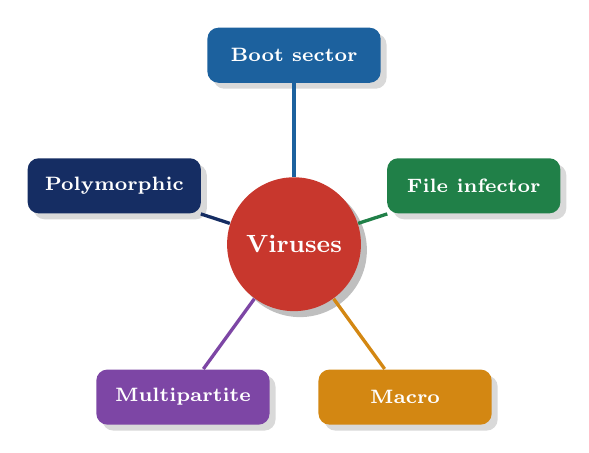
\begin{tikzpicture}
        \node[circle,fill=brick,text=white,font=\small\bfseries,minimum size=17mm,drop shadow] (c) at (0,0) {Viruses};
        \foreach \a/\t/\c in {90/Boot sector/ocean,18/File infector/leaf!80!black,-54/Macro/amber!90!black,-126/Multipartite/grape,162/Polymorphic/navy}{
          \node[solid box=\c,minimum width=22mm,minimum height=7mm,font=\scriptsize\bfseries] (s\a) at (\a:2.4) {\t};
          \draw[\c,very thick] (c) -- (s\a);
        }
      \end{tikzpicture}
    \end{column}
    \begin{column}{0.53\textwidth}
      {\small A true virus is code \textbf{inserted into other executable code}, so it runs whenever the program runs.}
      \begin{description}\small\setlength{\itemsep}{2pt}
        \item[\textcolor{ocean}{Boot sector}] Infect the DOS boot sector or master boot record; run at boot
        \item[\textcolor{leaf!70!black}{File infectors}] Attach to executables; run with the program
        \item[\textcolor{amber!80!black}{Macro}] Ride inside documents with macros; run when opened
        \item[\textcolor{grape}{Multipartite}] Combine boot sector + file infector
        \item[\textcolor{navy}{Polymorphic}] Change themselves on replication to dodge \textbf{signature} scanning
      \end{description}
    \end{column}
  \end{columns}
\end{frame}

% ------------------------------------------------------------
\begin{frame}{Worms, Trojans and Back Doors}
  \centering
  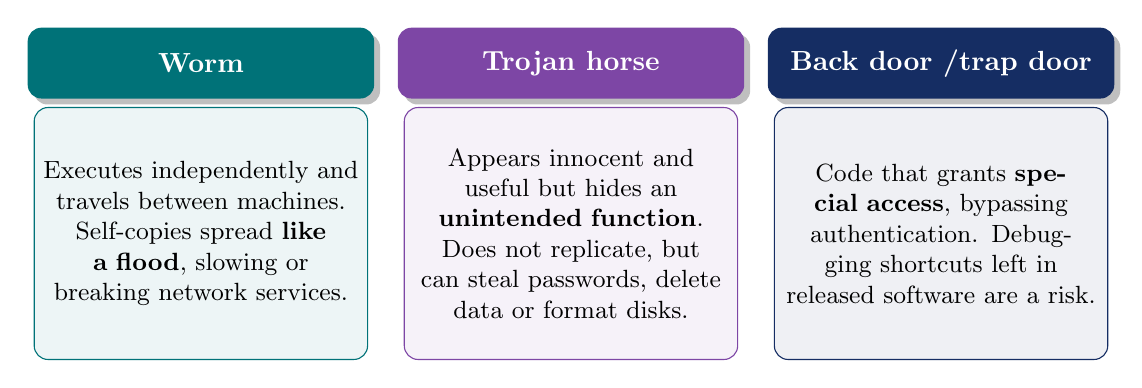
\begin{tikzpicture}
    \foreach \x/\c/\t/\d in {
      0/aqua!80!black/Worm/Executes independently and travels between machines. Self-copies spread \textbf{like a flood}\comma{} slowing or breaking network services.,
      4.7/grape/Trojan horse/Appears innocent and useful but hides an \textbf{unintended function}. Does not replicate\comma{} but can steal passwords\comma{} delete data or format disks.,
      9.4/navy/Back door \slash trap door/Code that grants \textbf{special access}\comma{} bypassing authentication. Debugging shortcuts left in released software are a risk.}
    {
      \node[fill=\c,text=white,rounded corners=5pt,font=\bfseries,minimum width=44mm,minimum height=9mm,drop shadow] (h) at (\x,0) {\t};
      \node[draw=\c,fill=\c!7,rounded corners=5pt,text width=40mm,minimum height=32mm,font=\small,anchor=north,align=center] at ([yshift=-1mm]h.south) {\d};
    }
  \end{tikzpicture}
\end{frame}

% ------------------------------------------------------------
\begin{frame}{Logic Bombs and Bacteria}
  \begin{columns}[T]
    \begin{column}{0.49\textwidth}
      \begin{block}{Logic bombs}
        \small Programmed threats that lie \textbf{dormant} in commonly used software for a long time until \textbf{pre-conditions} are met, such as a particular day. They come embedded in some programs.
      \end{block}
      \centering
      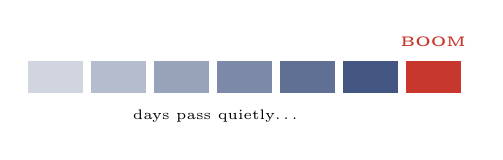
\begin{tikzpicture}
        \foreach \i in {0,...,5} \fill[navy!\the\numexpr 20+\i*12\relax] (\i*0.8,0) rectangle ++(0.7,0.4);
        \fill[brick] (4.8,0) rectangle ++(0.7,0.4);
        \node[font=\tiny\bfseries,text=brick] at (5.15,0.65) {BOOM};
        \node[font=\tiny] at (2.4,-0.3) {days pass quietly\dots};
      \end{tikzpicture}
    \end{column}
    \begin{column}{0.49\textwidth}
      \begin{alertblock}{Bacteria \slash rabbits}
        \small Do \textbf{not damage files}. Their aim is to \textbf{deny access} to resources by replicating until they consume all processor capacity, memory or disk space.
      \end{alertblock}
      \centering
      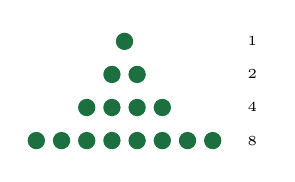
\begin{tikzpicture}
        \foreach \r/\n in {0/1,1/2,2/4,3/8}{
          \foreach \k in {1,...,\n} \fill[leaf!70!black] (\k*0.32-0.16*\n,-\r*0.42) circle (0.11);
          \node[font=\tiny,anchor=west] at (1.6,-\r*0.42) {\n};
        }
      \end{tikzpicture}
    \end{column}
  \end{columns}
\end{frame}

% ------------------------------------------------------------
\begin{frame}{Damage, Authors and Protection}
  \begin{columns}[T]
    \begin{column}{0.32\textwidth}
      \begin{alertblock}{Damage caused}
        \small Ranges from \textbf{merely annoying} to \textbf{catastrophic}: loss of data or services, disclosure of information. A software firm that ships malicious code risks its \textbf{reputation} and legal trouble.
      \end{alertblock}
    \end{column}
    \begin{column}{0.32\textwidth}
      \centering\textbf{\textcolor{brick}{Who writes virus code?}}\\[2mm]
      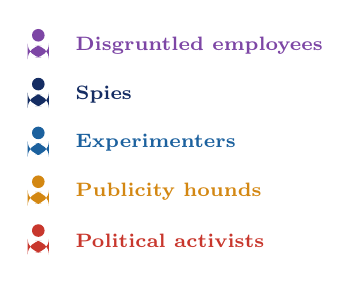
\begin{tikzpicture}
        \foreach \t/\c [count=\i from 0] in {Disgruntled employees/grape,Spies/navy,Experimenters/ocean,Publicity hounds/amber!90!black,Political activists/brick}{
          \pic[scale=0.5] at (0,-\i*0.62) {person=\c};
          \node[anchor=west,font=\scriptsize\bfseries,text=\c] at (0.35,-\i*0.62+0.1) {\t};
        }
      \end{tikzpicture}
    \end{column}
    \begin{column}{0.32\textwidth}
      \begin{exampleblock}{Protecting your system}
        \small
        \begin{itemize}\setlength{\itemsep}{2pt}
          \item Be careful about installing \textbf{new software}
          \item Never install binaries from \textbf{untrustworthy sources}
          \item Test new software first on a \textbf{non-critical system}
        \end{itemize}
      \end{exampleblock}
    \end{column}
  \end{columns}
\end{frame}

% ------------------------------------------------------------
\begin{frame}{Module 4 Summary}
  \begin{columns}[T]
    \begin{column}{0.49\textwidth}
      \begin{block}{What malicious software is}
        \small
        \begin{itemize}\setlength{\itemsep}{0pt}
          \item Perverse software and its motives
          \item Bombs, Trojans, worms, viruses (host? replicate?)
          \item Evolution: 1949 to Brain (1985)
          \item Booting, interrupts and ISRs
          \item Boot, system and .COM\slash.EXE infectors
          \item Famous viruses; four phases
        \end{itemize}
      \end{block}
    \end{column}
    \begin{column}{0.49\textwidth}
      \begin{exampleblock}{How we fight it}
        \small
        \begin{itemize}\setlength{\itemsep}{0pt}
          \item Precautions: prevention is better than cure
          \item Six anti-viral functions
          \item Damage control; no perfect anti-virus
          \item Hardening: Guest account, firewall, ports
          \item Six types of malicious code
        \end{itemize}
      \end{exampleblock}
    \end{column}
  \end{columns}
  \vspace{1mm}
  \begin{alertblock}{Review questions}
    \small
    1.~Define perverse software. \quad 2.~Explain the classification of viruses. \quad
    3.~Explain the different types of virus. \quad 4.~Write a short note on hardening network activity.
  \end{alertblock}
\end{frame}

% ------------------------------------------------------------
\begin{frame}{References}
  \begin{enumerate}\setlength{\itemsep}{8pt}
    \item William Stallings, \emph{Cryptography and Network Security}, PHI Publishers.
    \item Charlie Kaufman, Radia Perlman, \emph{Network Security}, Pearson Education.
    \item Bruce Schneier, \emph{Applied Cryptography}, John Wiley \& Sons.
    \item Roberta Bragg, \emph{Network Security: The Complete Reference}, TMH.
  \end{enumerate}
  \vspace{6mm}
  \centering
  
\begin{tikzpicture}
    \node[fill=navy,text=white,rounded corners=8pt,inner sep=10pt,font=\Large\bfseries,drop shadow] {Thank You! \; Questions?};
  \end{tikzpicture}
\end{frame}

\end{document}
